\chapter{Les Chambres à plaques résistives de CMS}
\renewcommand\chapterillustration{RPC/rpc}
\ThisULCornerWallPaper{1}{\chapterillustration}
\minitoc
\label{chap4}
\lettrine[lines=4, slope=-0.5em]{D}{ans} ce chapitre, une description générale des chambres à plaques résistives (RPC) ainsi qu'une description détaillée des chambres RPC utilisées dans CMS et de leurs électroniques sont données. Une description des mises à niveaux se rapportant à ces détecteurs, notamment dans les bouchons, sera également présentée.

\section{Les chambres à plaques résistives (RPC)}

 \marginpar
{
	\centering
	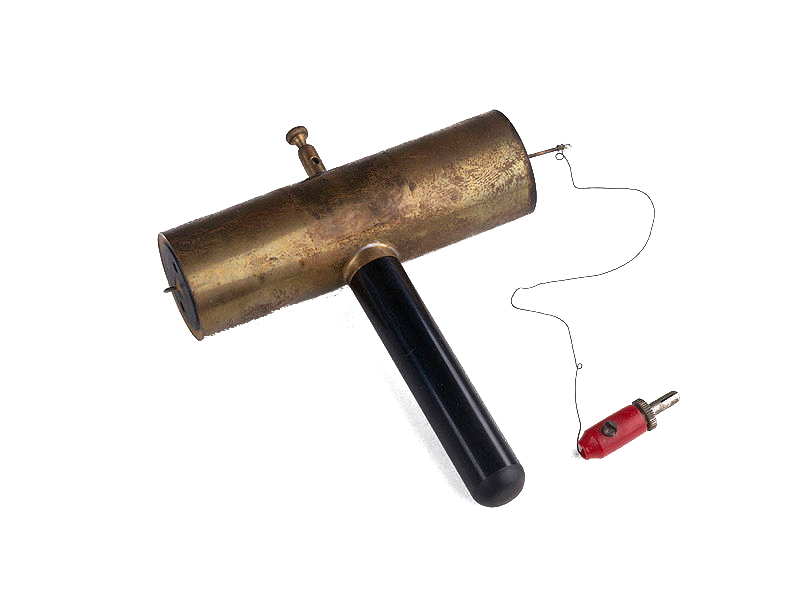
\includegraphics[width=\marginparwidth]{RPC/Geiger.png}
	\captionsetup{type=figure}\caption{Photo d'un des premiers tubes \bsc{Geiger}-\bsc{Müller} fabriqué en \num{1932} par \bsc{Hans Geiger} pour une utilisation en laboratoire.}
	\label{Geiger}
}
Les \textit{Resistive Plate Chambers} (RPC) font partie d'une famille de détecteurs appelée détecteurs gazeux. Ces détecteurs ont joué un rôle dès le début de la Physique des Hautes Énergies dans la détection de nouvelles particules. Depuis le premier détecteur gazeux, le compteur proportionnel à un seul fil \textit{Single-wire proportional counter} inventé par \bsc{Rutherford} et \bsc{Geiger}, puis le compteur \bsc{Geiger}-\bsc{Müller} (cf.Fig~\ref{Geiger}) présenté en \num{1928}, les détecteurs gazeux n'ont cessé de se perfectionner et de devenir plus rapides et efficaces. Ils permettent de couvrir de grandes surfaces de détections à des coûts très modestes.

\subsection{Les détecteurs gazeux}
Les détecteurs gazeux reposent tous sur le même principe simple. Lorsqu'une particule traverse un gaz, elle l'ionise. Les ions et électrons créés lors de cette ionisation peuvent être accélérés grâce à un champ électrique. En choisissant judicieusement l'intensité du champ électrique, c'est-à-dire en appliquant une tension aux bornes des électrodes, les électrons peuvent gagner assez d'énergie pour ioniser le gaz à leur tour (seconde ionisation) et commencer une multiplication de charge. Le nombre de charges libérées détermine le mode de fonctionnement du détecteur. Le gaz est également un élément important du détecteur et a un rôle important sur le mode de fonctionnement de celui-ci. Le déplacement des charges à l'intérieur du gaz induit un déplacement de charges sur les électrodes, et crée un signal qui peut être récupéré par une électronique et donner une information sur le temps et la position de la trajectoire de la particule incidente. Ces charges peuvent donner lieu à un mode dit \textit{"streamer"} voire donner lieu à la création d'étincelles entre l'anode et la cathode. La figure \ref{mult} montre le facteur d'amplification, ou le gain du gaz en fonction de la tension appliquée. 

\begin{figure}[ht!]
	\centering
	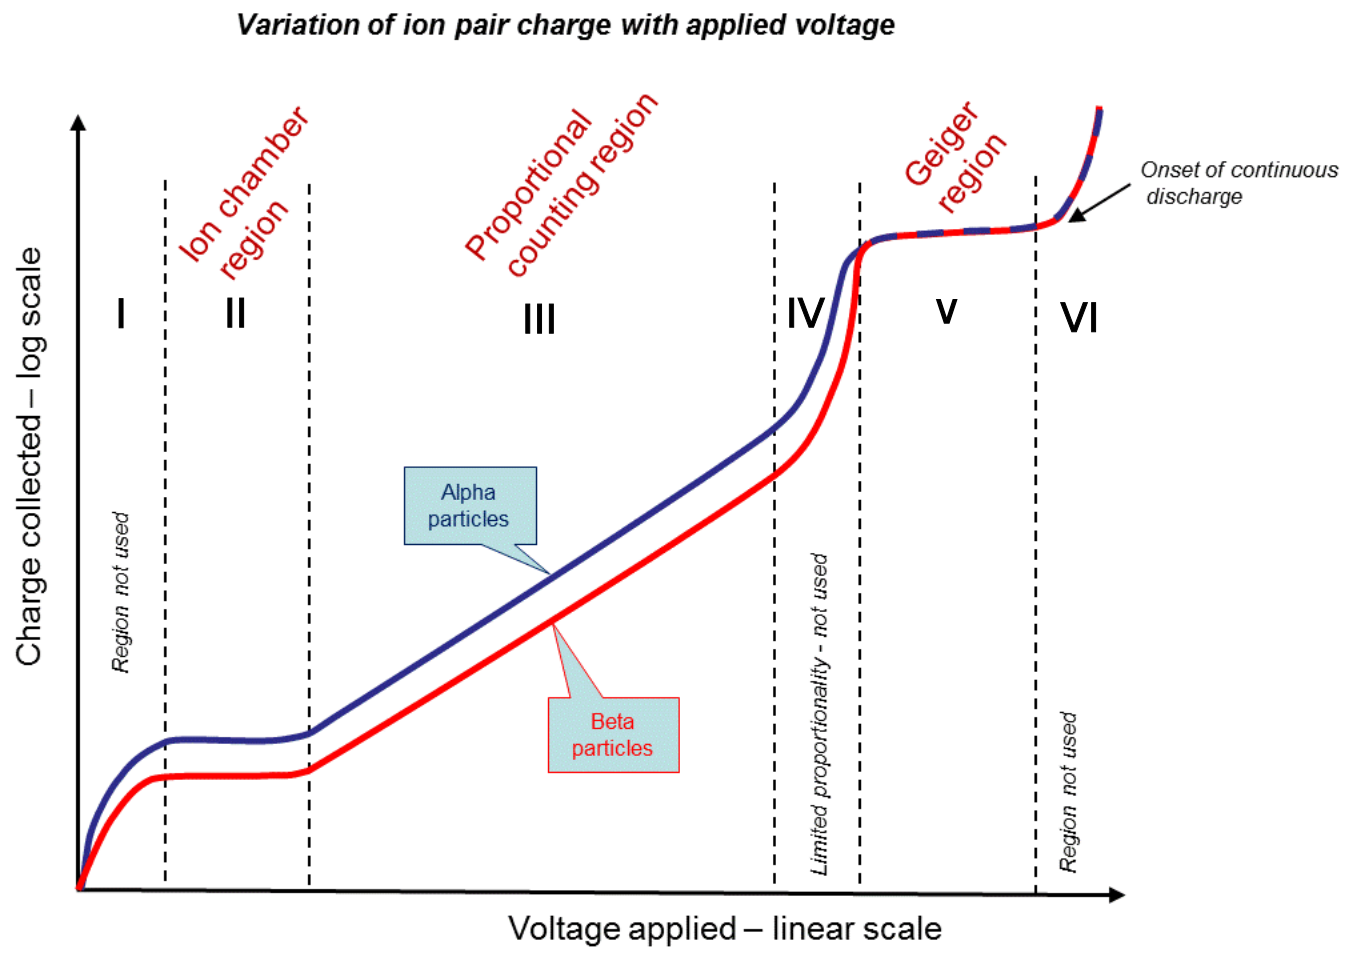
\includegraphics[width=0.98\textwidth]{RPC/gasgain.png}
	\captionsetup{type=figure}\caption{Évolution typique du gain du gaz en fonction de la tension appliquée (en échelle arbitraire).}
	\label{mult}
\end{figure}

Six régions peuvent être définies :

\begin{itemize}
	\item \textbf{I} Les paires d'électron-ion primaires se recombinent avant d'avoir été toutes récoltées.
	\item \textbf{II} Les charges dues à l'ionisation primaire sont entièrement récoltées sur les électrodes. Le facteur d'amplification reste constant même si la tension est augmentée.
	\item \textbf{III} Les charges produites par l'avalanche sont proportionnelles aux charges produites lors de la première ionisation. Les charges collectées augmentent fortement avec la tension appliquée.
	\item \textbf{IV} Cette région est la limite de proportionnalité, l'avalanche se transforme en \textit{streamer}, un plasma d'ions et d'électrons.
	\item \textbf{V} Les \textit{streamers} connectent les électrodes et produisent des étincelles visibles. Les compteurs \bsc{Geiger-Müller} et les chambres à étincelles fonctionnent dans ce mode.
	\item \textbf{VI} Des décharges électriques se produisent même sans le passage de particules pour ioniser le gaz. Ce mode peut détruire le détecteur.
\end{itemize}
\newpage
Les détecteurs gazeux à fils ont une résolution temporelle de l'ordre de la centaine de nanosecondes. Cela est dû au champ électrique en $\frac{1}{r}$, qui fait que la zone d'amplification se situe proche du fil, et les électrons doivent atteindre cette zone avant d'être amplifiés et de démarrer l'avalanche.

En utilisant un champ électrique uniforme et important, une meilleure résolution temporelle est atteignable.

Le premier détecteur gazeux utilisant cette méthode est le compteur à étincelle \textit{"Spark Counter"} développé en \num{1948}, un détecteur qui présente une géométrie plane. Il est généralement constitué de deux électrodes métalliques entre lesquelles est présent un gaz. Le passage d'une particule ionise ce gaz et crée une avalanche qui rentre à un certain moment en mode \textit{streamer}. Un plasma se crée entre les deux électrodes, celles-ci se déchargent et amènent à la création d'une étincelle. Ce type de détecteur présente un signal qui ne nécessite pas d'amplification, cependant le temps nécessaire à la recharge des électrodes est de l'ordre de quelques millisecondes. De plus la surface du détecteur ne doit pas être trop grande ($\sim\SI{10}{\square\centi\meter}$) afin de ne pas détruire les électrodes lors des décharges.

Afin de résoudre ces problèmes, les électrodes métalliques peuvent être remplacées par des plaques de matériaux de haute résistivité (\SIrange{1e11}{1e12}{\ohm\centi\meter}) afin de limiter l'aire de décharge des électrodes autour du signal. Un mélange de gaz absorbant les photons permet d'éviter le mode \textit{streamer}, assurant le fonctionnement du détecteur à des flux de particules plus important. Le champ électrique baissant localement du fait de la recharge plus lente des électrodes, le développement d'avalanches successives au même endroit est limité tout en laissant le détecteur opérationnel hors de cette zone.
\vspace{-0.4cm}
\subsubsection{Naissance des RPC}
\vspace{-0.4cm}
En \num{1981} \bsc{R.Santonico} et \bsc{R.Cardarelli} développent les \textit{Resistive Plate Chamber} (RPC) \cite{Santonico:1981sc} \cite{CARDARELLI198820}. Ce détecteur utilise un matériau peu coûteux, très utilisé et de haute résistivité ($\sim$\SI{e10}{\ohm\centi\meter}), le \textit{High Pressure Laminate} (HPL) fait de mélamine ou d'un type de résine phénol-formaldéhyde (anhydrure de polyoxybenzylméthylèneglycol ou Bakélite (cf.Fig~\ref{bakelite})). 
\marginpar
{
	\centering
	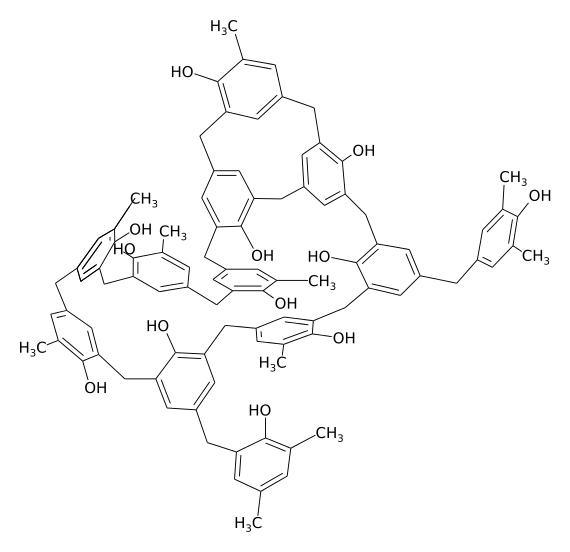
\includegraphics[width=\marginparwidth]{RPC/bakelite.png}
	\captionsetup{type=figure}\caption{Structure de la Bakélite.}
	\label{bakelite}
}
Plusieurs configurations pour les RPC sont possibles, mais l'une des plus simples est donnée par la figure \ref{RPCscheme}.

\begin{figure}[th!]
	\centering
	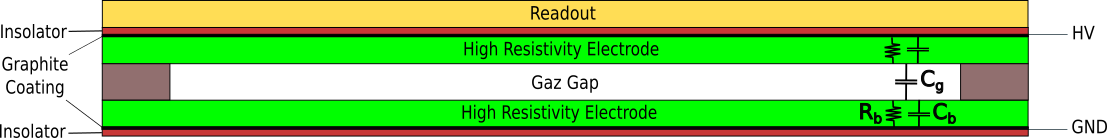
\includegraphics[width=0.95\textwidth]{RPC/scheme_first.png}
	\captionsetup{type=figure}\caption{Schéma d'une RPC typique.}
	\label{RPCscheme}
\end{figure}
\vspace{-0.1cm}
Une couche de gaz est comprise entre deux plaques d'électrodes résistives. Ces plaques sont peintes avec du graphite qui est utilisé pour distribuer la haute tension sur les électrodes. L'électronique est isolée de la chambre par un isolant fin, de type feuille de poly(téréphtalate d'éthylène) (Mylar). L'électronique peut être placée de chaque coté de la chambre et peut être constituée de carreaux ou de lamelles etc.

Un modèle électrique simplifié d'une RPC peut être obtenu (cf.Fig~\ref{RPCscheme}) en notant $C_{b}$ la capacité de la Bakélite, $R_{b}$ sa résistance et $C_{g}$ la capacité du gaz.

La résistance de la Bakélite est donnée par :
\begin{equation}
R_b=\frac{\rho d}{S}
\end{equation}
avec $\rho$ la résistivité de la Bakélite, $d$ l'épaisseur de l'électrode et $S$ sa surface.

La capacité de la Bakélite est donnée quant à elle par :
\begin{equation}
C_{b}=\epsilon_0\epsilon_r\frac{S}{d}
\end{equation} 
avec $\epsilon_0$ la permittivité du vide et $\epsilon_r$ la permittivité relative de la Bakélite.

Le temps de décharge $\tau$ d'une électrode de telle résistivité et de telle capacité recevant une charge $Q_{0}$ peut être obtenu en utilisant la formule :
\begin{equation}
Q(t)=Q_{0}e^{\frac{-t}{R_bC_b}}=Q_{0}e^{\frac{-t}{\rho\epsilon_{0}\epsilon_{r}}}=Q_{0}e^{\frac{-t}{\tau}}
\end{equation}
Les charges présentes sur les électrodes réduisent la haute tension appliquée et donc le champ électrique à l'endroit des charges. Le détecteur devient inefficace pour cette période de temps $\tau$ à l'endroit du dépôt des charges tout en restant efficace ailleurs. Pour le cas de la Bakélite $\rho\simeq\SI{1e11}{\ohm\centi\meter}$ le temps de relaxation est de l'ordre de \SI{10}{\milli\second}. Grâce à l'emploi de matériaux de haute résistivité, l'utilisation de chambres de grande taille était désormais possible.


Depuis, ces détecteurs de construction simple et robuste ont été utilisés dans de nombreuses expériences : ATLAS \cite{ATLAS}, BaBar \cite{Boutigny:1995ib} (cf.Fig~\ref{babar}), BELLE \cite{ABASHIAN2002117} (cf.Fig~\ref{belle}),  \textit{Oscillation Project with Emulsion-tRacking Apparatus} (OPERA) \cite{1748-0221-9-10-C10003} (cf.Fig~\ref{opera}) etc. Différentes solutions technologiques ont été développées en fonction des besoins des différentes expériences.

\marginpar
{
	\centering
	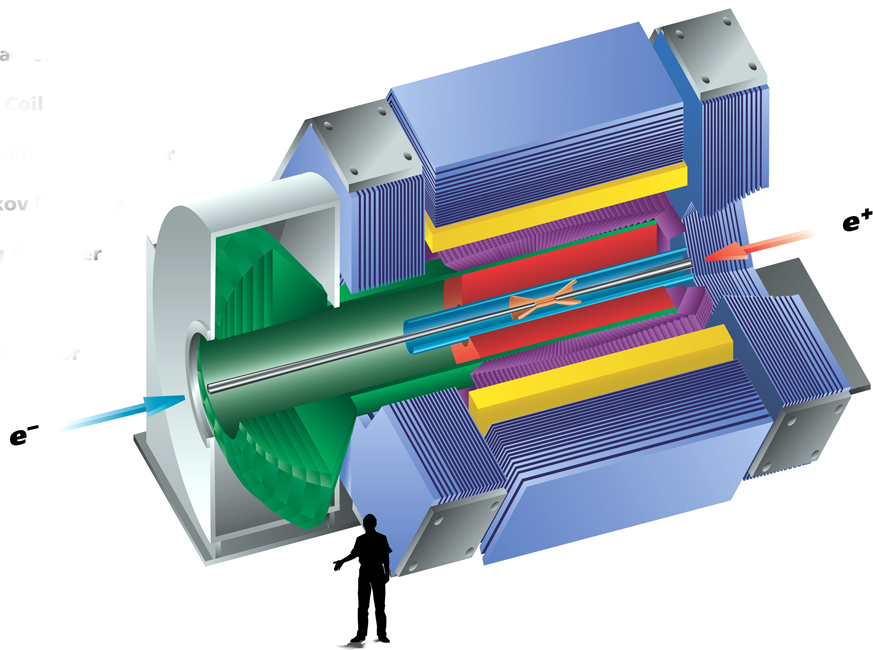
\includegraphics[width=\marginparwidth]{RPC/babar.png}
	\captionsetup{type=figure}\caption{Schéma de l'expérience BaBar.}
	\label{babar}
}

\marginpar
{
	\centering
	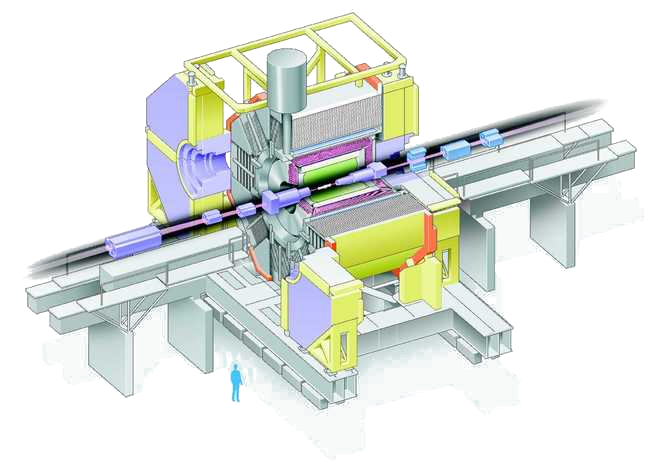
\includegraphics[width=\marginparwidth]{RPC/belle.png}
	\captionsetup{type=figure}\caption{Schéma de l'expérience BELLE.}
	\label{belle}
}

\marginpar
{
	\centering
	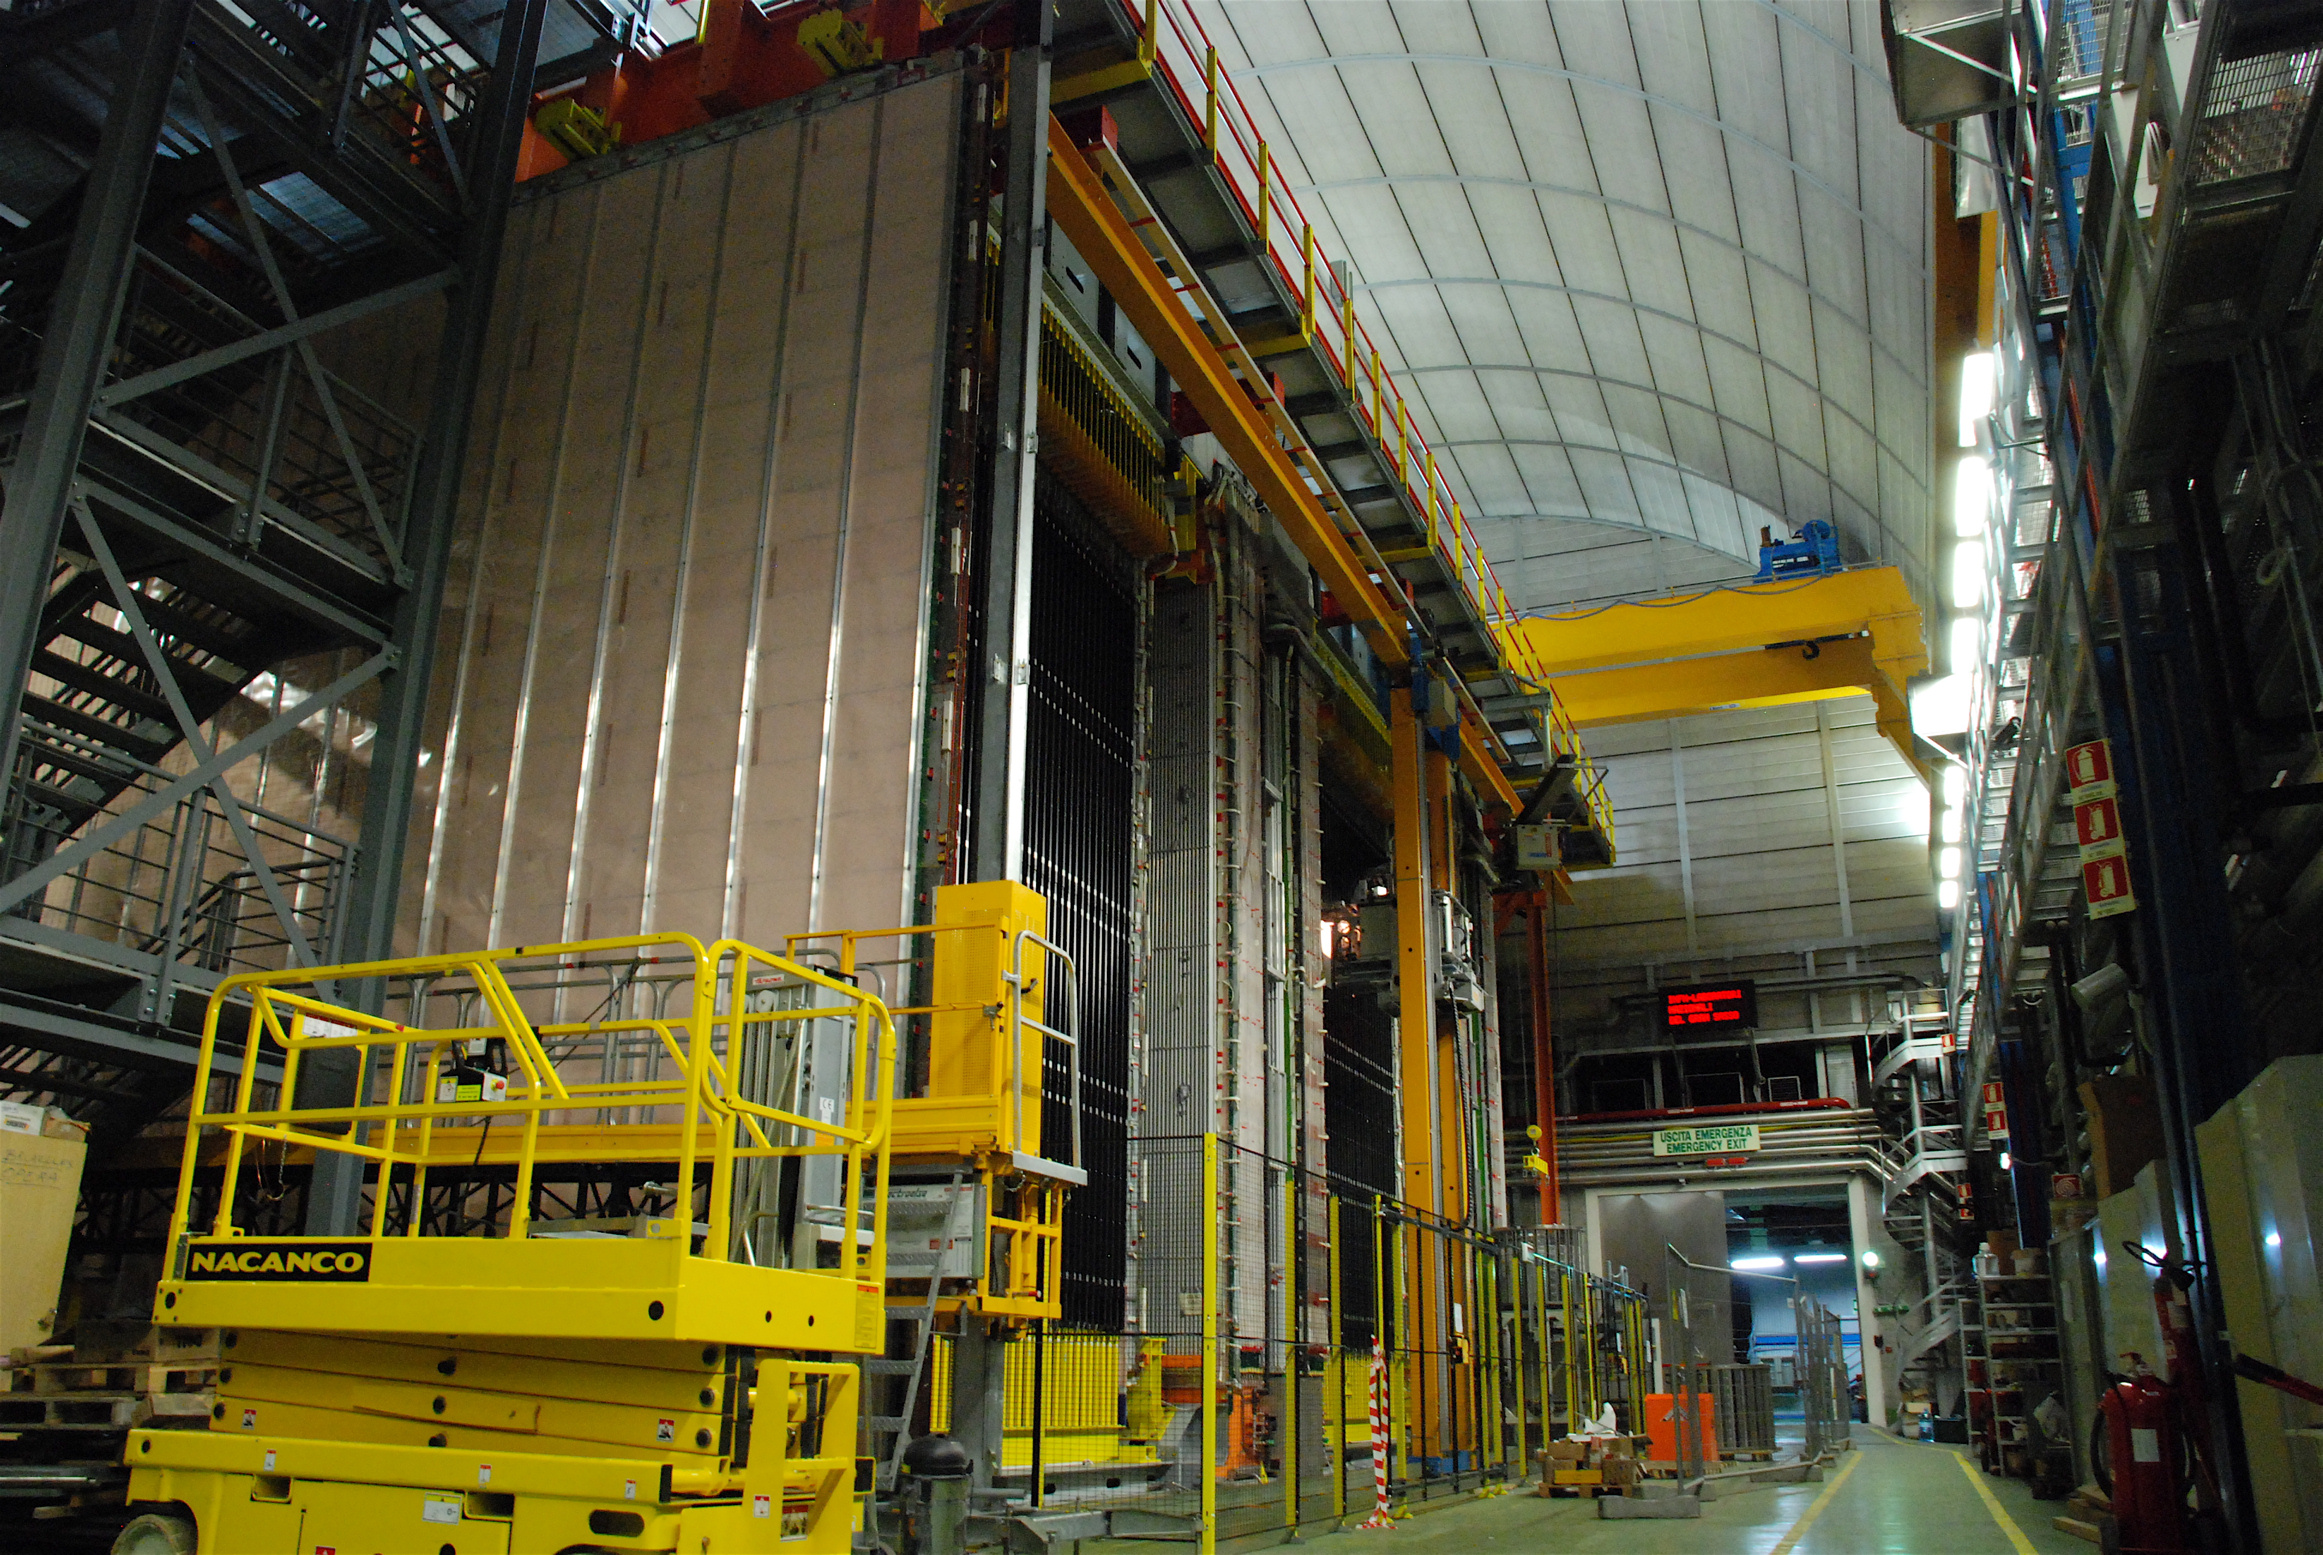
\includegraphics[width=\marginparwidth]{RPC/OPERA.jpg}
	\captionsetup{type=figure}\caption{Photo du détecteur OPERA.}
	\label{opera}
}

\subsection{Principes de fonctionnement d'une RPC}
Le principe d'une RPC repose sur l'ionisation d'un gaz. Lorsqu'une particule relativiste traverse le gaz d'une RPC, elle interagit avec les molécules de gaz principalement par interaction électromagnétique. La perte d'énergie moyenne par ionisation et excitation d'une particule relativiste massive ($m>m_{e}$) due à des électrons libres supposés au repos est donnée par la formule de \bsc{Bethe}-\bsc{Bloch} (cf.fig\ref{Bethe-Block})
\begin{equation}
-\left<\frac{1}{\rho}\frac{\dd E}{\dd x}\right>=\frac{e^{4}}{4\pi \epsilon_{0}^{2}m_{e}c^{2}}z^{2}N_{A}\frac{Z}{A}\frac{1}{\beta^{2}}\left[\frac{1}{2}\ln\frac{2m_{e}c^{2}\beta^{2}\gamma^{2}E_{max}}{I^{2}}-\beta^{2}-\frac{\delta(\beta\gamma)}{2}\right]
\end{equation}
avec :

\begin{itemize}[label=$\bullet$]
	\item $\rho$ la densité du matériau,
	\item $e$ la charge de l'électron,
	\item $\epsilon_{0}$ la permittivité du vide,
	\item $c$ la vitesse de la lumière dans le vide,
	\item $z$ la charge de la particule incidente,
	\item $N_{A}$ le nombre d'\bsc{Avogadro},
	\item $Z$ le numéro atomique du matériau,
	\item $A$ le nombre de masse du matériau,
	\item $\beta=\frac{v}{c}$ la vitesse de la particule incidente en unité de $c$,
	\item $\gamma=\frac{1}{\sqrt{1-\beta^{2}}}$,
	\item $I$ est l'énergie d'excitation moyenne,
	\item $E_{max}$ est l'énergie maximale transférée lors d'une collision d'une particule de masse $m$ et de quantité de mouvement $p$,
	\begin{equation}
	E_{max}=\frac{2m_{e}p^{2}}{m^2+2\gamma m_{e}m+m_{e}^2}
	\end{equation}
\end{itemize}

\begin{minipagewithmarginpars}[h]{0.95\textwidth}
	\centering
	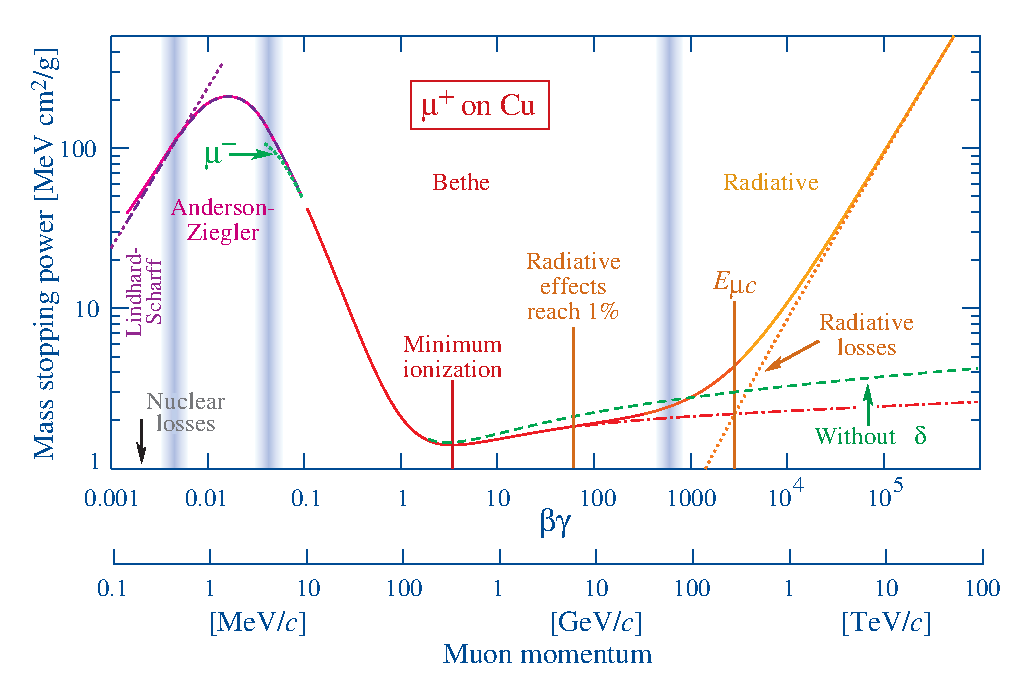
\includegraphics[width=0.70\textwidth]{RPC/Bethe-Bloch.eps}
	\captionsetup{type=figure}\caption{Perte d'énergie moyenne $-\left<\frac{\dd E}{\dd x}\right>$ pour des anti-muons dans du cuivre en fonction de $\beta\gamma=\frac{p}{Mc}$ sur neuf ordres de grandeur en quantité de mouvement (douze ordres de grandeur en énergie cinétique)\cite{Olive:2016xmw}.}
	\label{Bethe-Block}
\end{minipagewithmarginpars}

\marginpar
{
	\centering
	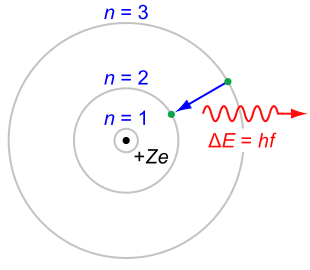
\includegraphics[width=\marginparwidth]{RPC/Photon.png}
	\captionsetup{type=figure}\caption{Émission d'un photon lors de la désexcitation d'un atome.}
	\label{photon}
}
\marginpar
{
	\centering
	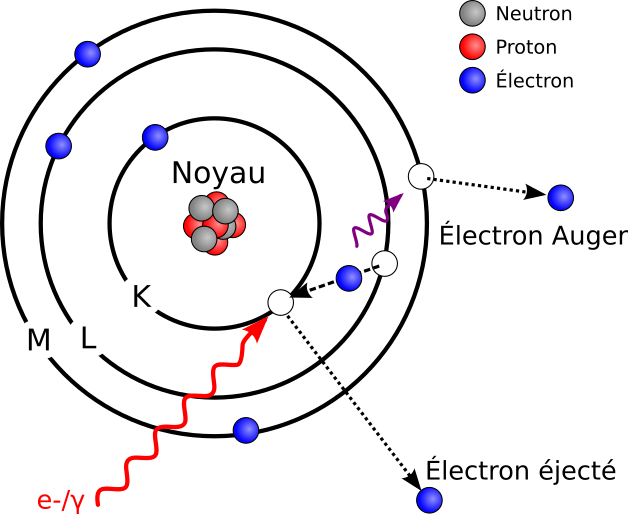
\includegraphics[width=\marginparwidth]{RPC/Auger.png}
	\captionsetup{type=figure}\caption{Éjection d'un électron Auger.}
	\label{Auger}
}
\marginpar
{
	\centering
	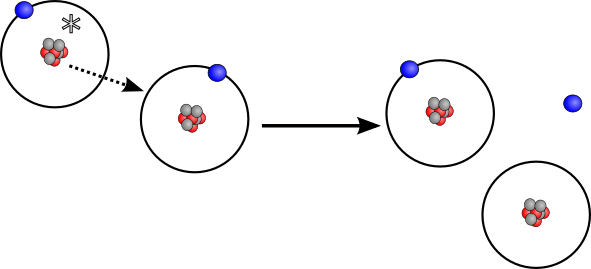
\includegraphics[width=\marginparwidth]{RPC/Penning.png}
	\captionsetup{type=figure}\caption{Ionisation Penning.}
	\label{Penning}
}
\marginpar
{
	\centering
	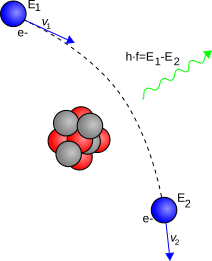
\includegraphics[width=\marginparwidth]{RPC/Brem.png}
	\captionsetup{type=figure}\caption{Bremsstrahlung produit par un électron dévié par le champ électrique d'un noyau.}
	\label{Brem}
}

Si un atome ou une molécule du gaz est ionisé par la collision inélastique de la particule incidente, des électrons sont éjectés de l'atome près du point de collision. En revanche, si l'atome n'est pas ionisé mais excité, l'énergie d'excitation est évacuée par l'émission d'un photon (cf.Fig~\ref{photon}), par un électron \bsc{Auger} (cf.Fig~\ref{Auger}) ou par ionisation \bsc{Penning} (cf.Fig~\ref{Penning}). Si ce photon a une énergie plus importante que le minimum du potentiel d'ionisation, le photon va être absorbé par effet photoélectrique et un électron va être éjecté de l'atome, sinon le photon ne sera pas détecté par les RPC.

Une particule chargée relativiste peut aussi perdre son énergie par rayonnement continu de freinage appelé \textit{Bremsstrahlung} (cf.Fig~\ref{Brem}), ce processus devient prédominant si l'énergie de la particule dépasse une certaine énergie critique ($E_{\mu c}$ sur la figure \ref{Bethe-Block}). Dans ce cas, la perte d'énergie n'est pas détectée par la RPC.

Le fonctionnement d'une RPC repose sur la perte d'énergie par ionisation et excitation. Cette perte d'énergie dépend du matériau (cf.Fig~ \ref{mat}). Lors de l'ionisation du gaz, des amas primaires (d'électrons et ions) sont créés le long de la trajectoire de la particule incidente. 


\begin{figure}[ht!]
	\centering
	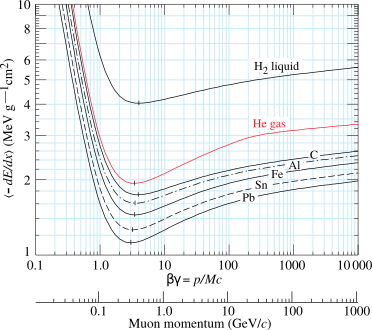
\includegraphics[width=0.55\textwidth]{RPC/energylost.png}
	\captionsetup{type=figure}\caption{Perte d'énergie moyenne dans l'hydrogène liquide, l'hélium liquide, le carbone, l'aluminium, le fer, l'étain et le plomb. Les effets radiatifs, pertinents pour les pions et muons, ne sont pas inclus. Ils deviennent importants pour les muons traversant le fer avec $\beta\gamma\gtrsim1000$ et à plus petite quantité de mouvement pour les muons dans des absorbeurs de plus grand $Z$ \cite{Olive:2016xmw}.}
	\label{mat}
\end{figure}

\subsection{Les modes de fonctionnement des RPC}

Selon l'intensité du champ électrique appliqué entre les électrodes, il est possible de choisir le mode de fonctionnement des chambres. La composition du mélange gazeux est également un élément déterminant. On distingue généralement trois modes de fonctionnement : le mode avalanche, le mode \textit{streamer} et le mode éclair (\textit{spark}).

\subsubsection{Le mode avalanche}

Le mode avalanche est le premier mode de fonctionnement qui apparaît lorsqu'on augmente la tension entre les électrodes. L'ionisation du gaz crée quelques paires d'ion-électron qui sont ensuite accélérées par le champ électrique. Les électrons, qui sont beaucoup plus rapides que les ions de par leur masse plus faible vont à leur tour ioniser les molécules du gaz. Cette multiplication des charges est appelée avalanche. Ce déplacement va créer par effet capacitif un signal de l'ordre de la nanoseconde qui peut être récolté. Les charges vont ensuite atteindre les électrodes et s'y accumuler. Elles vont être neutralisées en quelques millisecondes grâce au courant fourni par le générateur de haute tension appliquant la différence de potentiel (cf.Fig~\ref{avalanche}). Le temps mort de ce mode est donc assez faible et permet une détection efficace des particules même à des flux assez élevés ($\sim\SI{1}{\kilo\hertz}$), la résistivité du matériau est déterminante pour ce temps de neutralisation des charges. Cependant, la charge induite est faible et nécessite une électronique possédant un bas seuil et donc de bas bruit.

\begin{figure}[ht!]
\centering
\subfloat[Des molécules du gaz sont ionisées par le passage d'une particule.]{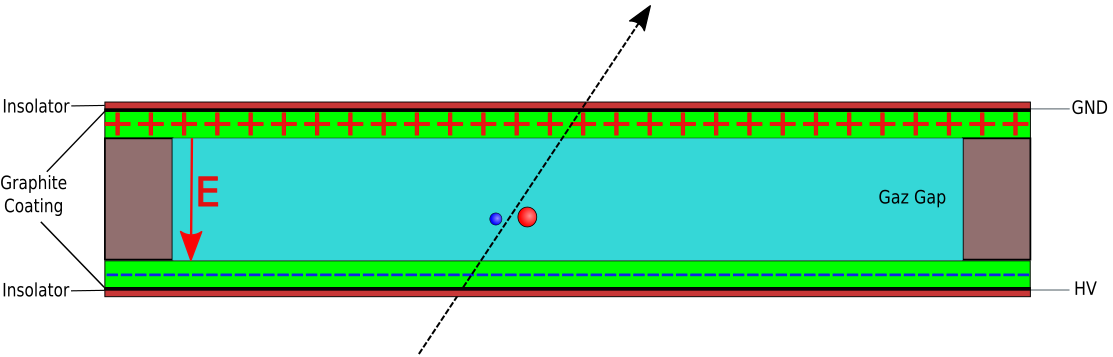
\includegraphics[width=.49\linewidth]{RPC/avalanche-streamer-1.png}\label{avalanche-1}}
\hfill
\subfloat[La taille de l'avalanche influence le champ électrique local de la couche de gaz.]{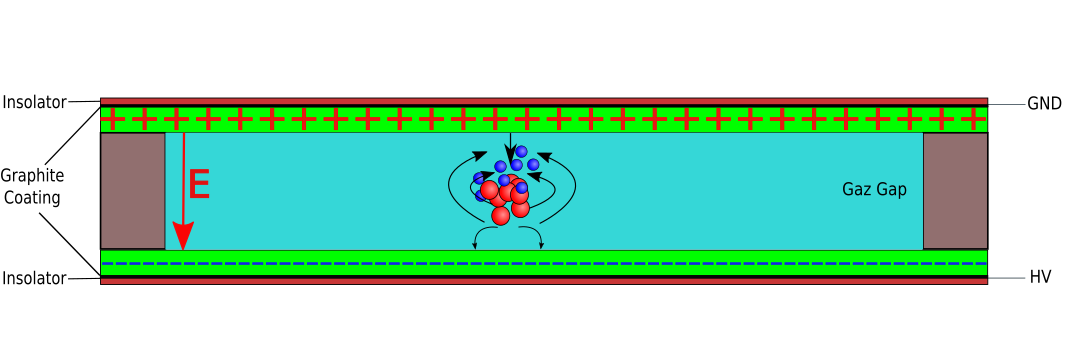
\includegraphics[width=.49\linewidth]{RPC/avalanche-2.png}\label{avalanche-2}}
\\
\subfloat[Les électrons atteignent l'anode. Les ions sont beaucoup plus lents.]{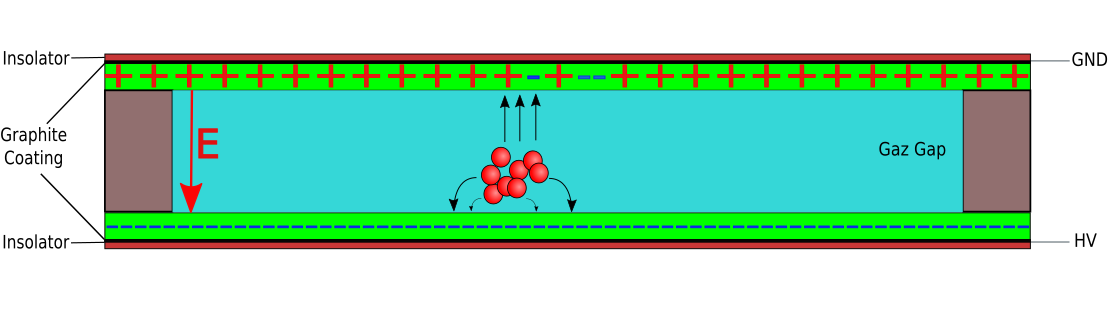
\includegraphics[width=.49\linewidth]{RPC/avalanche-3.png}\label{avalanche-3}}
\hfill
\subfloat[Les ions atteignent la cathode. Les charges de la couche résistive induisent un temps mort.]{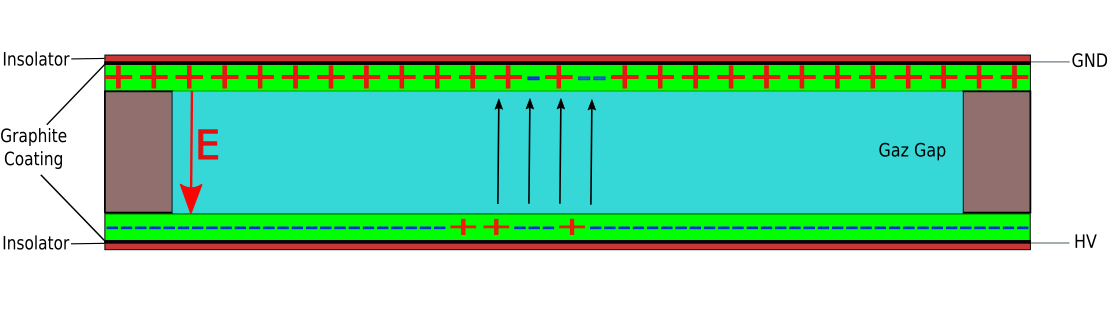
\includegraphics[width=.49\linewidth]{RPC/avalanche-4.png}\label{avalanche-4}}
\caption{Vue schématique du développement d'une avalanche. Le champ électrique appliqué aux électrodes est noté $E$, les électrons sont en bleu et les ions en rouge.}
\label{avalanche}
\end{figure}

\subsubsection{Le mode \textit{streamer}}

Si l'on augmente la tension aux bornes des électrodes, le gain du gaz augmente, ainsi les ionisations primaires créent plus d'ionisations secondaires. Il y a donc création de paires électron-ion en plus grand nombre. De plus les photons peuvent commencer à contribuer à la propagation de l'avalanche, ce qui amène au mode \textit{streamer}. Le signal engendré par ce mode est plutôt important (de \SI{50}{\pico\coulomb} à quelques \si{\nano\coulomb}), de fait l'électronique ne nécessite pas d'amplification et est beaucoup plus simple. Cependant, le flux de particules maximal est limité à quelques centaines de Hertz. Si les électrons deviennent trop nombreux (en moyenne $10^{8}$ électrons), ils engendrent un plasma reliant les deux électrodes (cf.Fig~ \ref{streamer}).

\begin{figure}[ht!]
	\centering
	\subfloat[Des molécules du gaz sont ionisées par le passage d'une particule.]{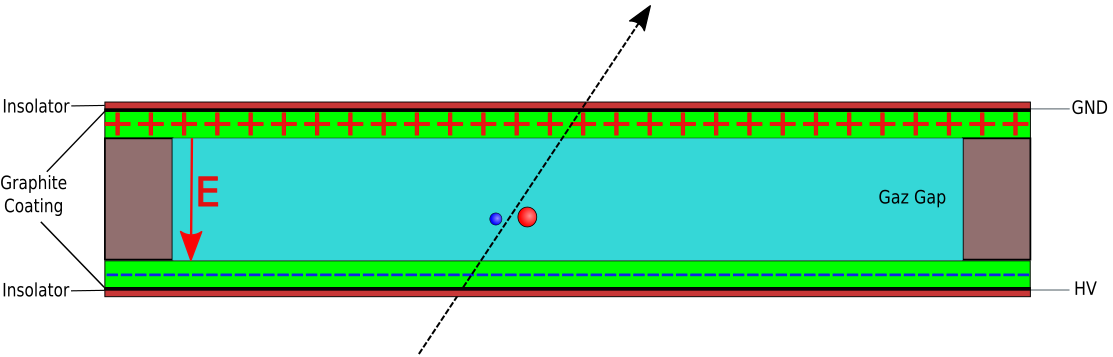
\includegraphics[width=.49\linewidth]{RPC/avalanche-streamer-1.png}\label{streamer-1}}
	\hfill
	\subfloat[La taille de l'avalanche modifie fortement le champ électrique local de la couche de gaz. ]{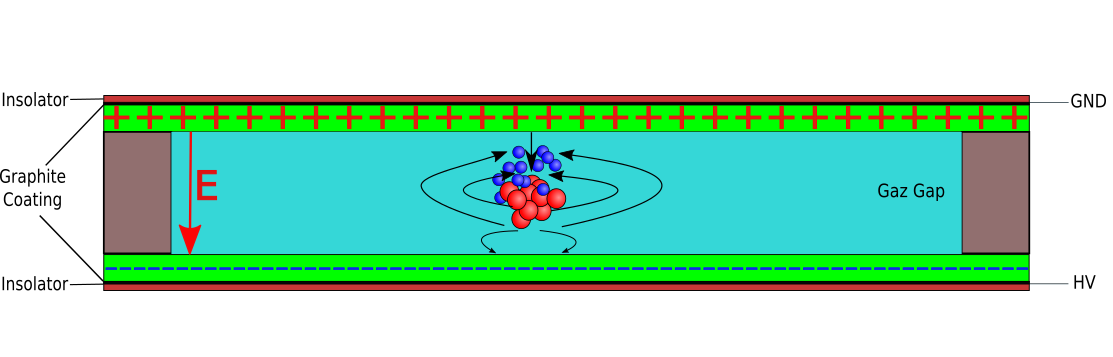
\includegraphics[width=.49\linewidth]{RPC/streamer-22.png}\label{streamer-2}}
	\\
	\subfloat[Les photons contribuent au développement de l'avalanche et étalent l'avalanche. Passage au mode \textit{streamer}.]{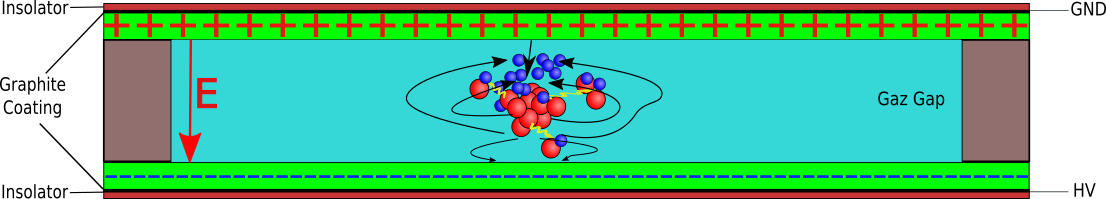
\includegraphics[width=.49\linewidth]{RPC/streamer-3.png}\label{streamer-3}}
	\hfill
	\subfloat[Les charges de la couche résistive induisent un temps mort important.]{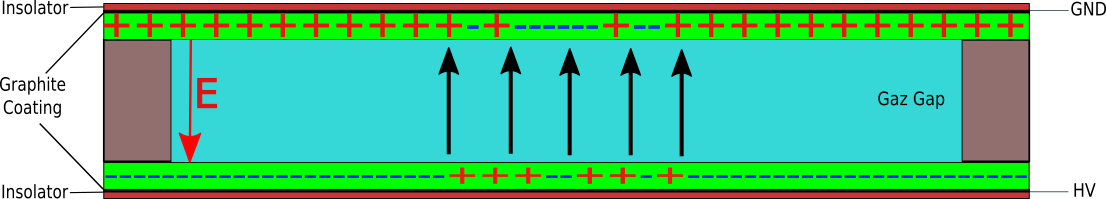
\includegraphics[width=.49\linewidth]{RPC/streamer-5.png}\label{streamer-5}}
	\caption{Vue schématique du développement d'un \textit{streamer}. Le champ électrique appliqué aux électrodes est noté $E$, les électrons sont en bleu et les ions en rouge.}
	\label{streamer}
\end{figure}

\subsubsection{Le mode éclair (\textit{spark})}
Si l'on augmente encore la tension ou si le mélange de gaz ne permet pas de limiter la propagation latérale de l'avalanche ou le mode \textit{streamer}, les électrons migrateurs et les photons peuvent induire de proche en proche d'autres \textit{streamers}, c'est le mode éclair, ou \textit{spark}. Les éclairs se propagent alors dans toute la chambre. Le temps de recouvrement de la chambre devient très long et les charges accumulées peuvent détériorer rapidement le détecteur. De plus le flux de particules détectable est très faible (cf.Fig~ \ref{spark}).
\begin{figure}[ht!]
	\centering
	\subfloat[Des molécules du gaz sont ionisées par le passage d'une particule.]{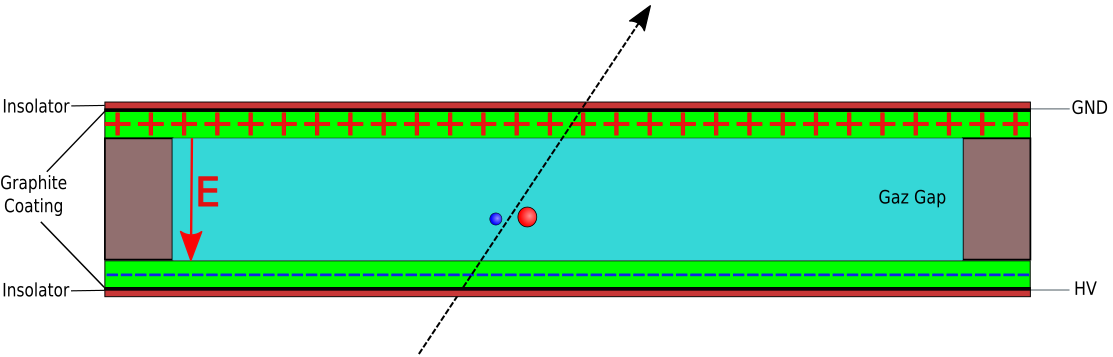
\includegraphics[width=.49\linewidth]{RPC/avalanche-streamer-1.png}\label{spark-1}}
	\hfill
	\subfloat[La taille de l'avalanche modifie fortement le champ électrique local de la couche de gaz. ]{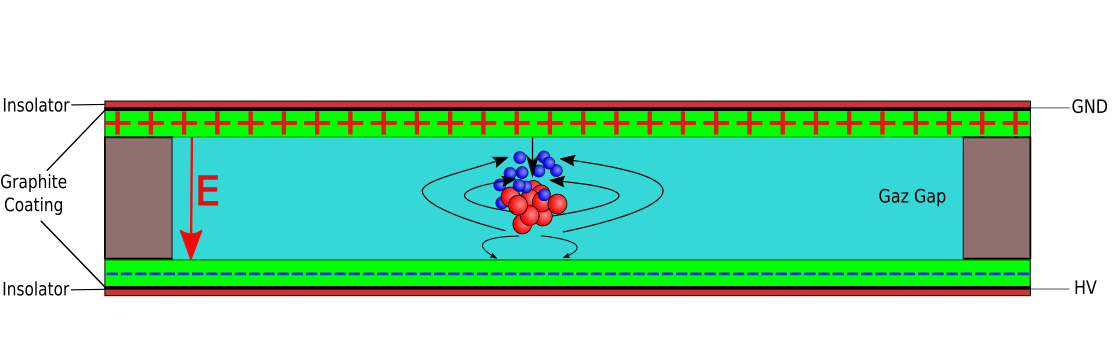
\includegraphics[width=.49\linewidth]{RPC/spark-2.png}\label{spark-2}}
	\\
	\subfloat[Les photons contribuent au développement de l'avalanche et étalent l'avalanche. Passage au mode \textit{streamer}.]{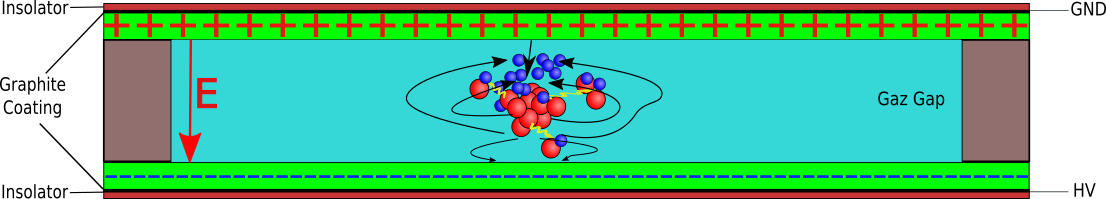
\includegraphics[width=.49\linewidth]{RPC/streamer-3.png}\label{spark-3}}
	\hfill
	\subfloat[Un plasma peut se créer entre les électrodes et produire une étincelle. Les electrodes sont déchargées à cet endroit (mode éclair).]{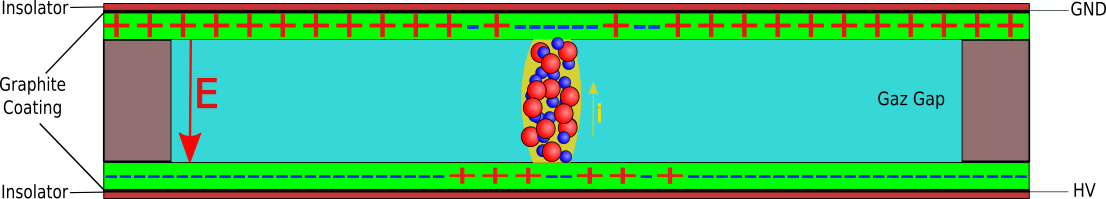
\includegraphics[width=.49\linewidth]{RPC/streamer-4.png}\label{spark-4}}
    \\
	\subfloat[Des éclairs se créent de proche en proche à cause des électrons migrateurs et des photons.]{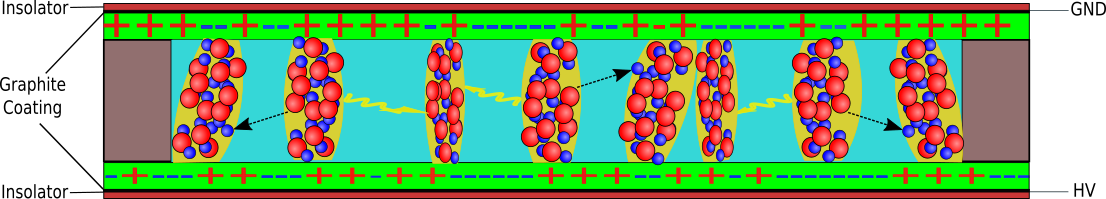
\includegraphics[width=.49\linewidth]{RPC/spark-5.png}\label{spark-5}}
    \hfill
	\subfloat[Le champ électrique est fortement abaissé dans toute la chambre. Elle est aveugle.]{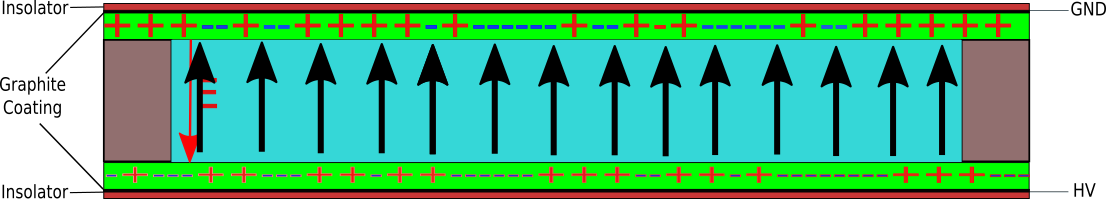
\includegraphics[width=.49\linewidth]{RPC/spark-6.png}\label{spark-6}}
	\caption{Vue schématique du développement d'un \textit{spark}. Le champ électrique appliqué aux électrodes est noté $E$, les électrons sont en bleu et les ions en rouge.}
	\label{spark}
\end{figure}


Dans CMS le mélange de gaz ainsi que les tensions appliquées ont été judicieusement étudiés pour que les RPC soient le plus possible en mode avalanche afin de maximiser le flux de particules que peuvent détecter les chambres tout en évitant leur vieillissement prématuré. C'est donc ce mode que nous allons étudier plus avant.

\subsection{Étude théorique du mode avalanche}

\subsubsection{Ionisation primaire}
Le mélange gazeux des détecteurs contient majoritairement un gaz à faible potentiel d'ionisation minimale afin d'être facilement ionisable. En pratique, la plupart des détecteurs utilisent du tétrafluoroéthylène (\chemform{TFE}) de potentiel d'ionisation minimal $U_{i}=\SI{10.114 \pm0.010}{\eV}$ \cite{Chimie:chimie}. La création de charges primaires dues au passage d'une particule chargée dans le mélange de gaz est caractérisée par le nombre moyen d'amas créés par unité de longueur ainsi que par le nombre de paires électron-ion créées dans chaque amas.

\subsubsection{Distance entre les amas de l'ionisation primaire}
Si l'on considère que l'énergie perdue dans le matériau par la particule incidente est négligeable par rapport à son énergie initiale, alors les probabilités de collisions ionisantes sont indépendantes. Les distances entre les amas d'ionisations primaires suivent donc une loi exponentielle :
\begin{equation}
P(z)=\frac{1}{L}\exp\left(-\frac{z}{L}\right)
\end{equation} 
où $L$ est le libre parcours moyen et $z$ l'épaisseur à laquelle l'ionisation a lieu en considérant des particules incidentes dont la trajectoire est normale au plan du détecteur. Pour des particules incidentes d'angle $\phi$ par rapport à l'axe $z$ la formule devient:
\begin{equation}
P(z)=\frac{1}{L}\exp\left(-\frac{z}{L\cos\phi}\right)
\end{equation}
La distance moyenne entre les amas primaires peut se calculer en utilisant le programme de simulation Monte-Carlo HEED \cite{HEED}. Une comparaison entre les mesures et les simulations pour l'isobutane et le méthane est donnée figure \ref{lambda} et montre de bons accords \cite{2004NIMPA}.  

\begin{figure}[ht!]
	\centering
	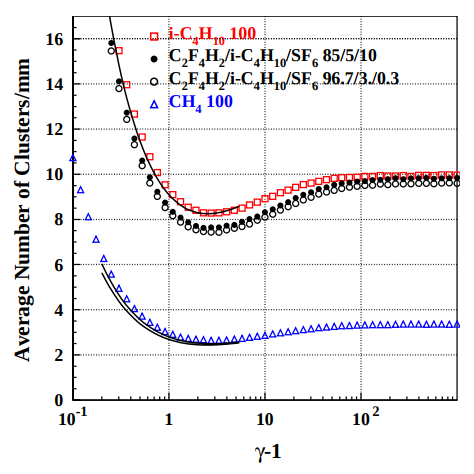
\includegraphics[width=0.60\textwidth]{RPC/lambda.png}
	\captionsetup{type=figure}\caption{Nombre de collisions donnant lieu à des ionisations (nombre d'amas) par \si{\milli\meter} en fonction de $\gamma-1$, avec $\gamma=\frac{1}{\sqrt{1-\beta^{2}}}$, pour différents mélanges de gaz, tel que prédit par HEED \cite{HEED}, avec $T=\SI{296.15}{\kelvin}$ et $p=\SI{1013}{\milli\bar}$. Les lignes correspondent à des mesures prises de \cite{PhysRevA.6.1507}.  }
	\label{lambda}
\end{figure}

Le nombre moyen d'amas contenus dans une couche de gaz d'épaisseur $e$ est donc $\bar{n}=\frac{e}{L}$. La probabilité d'avoir $n$ amas dans cette couche de gaz suit une loi de \bsc{Poisson} :
\begin{equation}
P(n)=\frac{1}{n!}\left(\frac{e}{L}\right)^{n}\exp\left(-\frac{e}{L}\right).
\end{equation}
En supposant un détecteur parfait, l'efficacité maximale pour une chambre d'épaisseur $e$ est donnée par :
\begin{equation}
\epsilon_{max}=1-P(0)=1-\exp\left(-\bar{n}\right)
\end{equation}
où $P(0)$ est la probabilité qu'aucune ionisation ne soit créée dans l'épaisseur de gaz de la chambre.

\subsubsection{Nombre d'électrons dans les amas primaires}
Le nombre d'électrons par amas d'ionisation primaire est variable et dépend de l'énergie échangée entre le gaz et la particule incidente. La distribution du \textit{"cluster size"} a été calculée par \bsc{Riegler} et al. \cite{Riegler:570462} en utilisant HEED pour des mélanges de gaz très utilisés par les RPC (cf.Fig~\ref{cluster})
\begin{figure}[ht!]
	\centering
	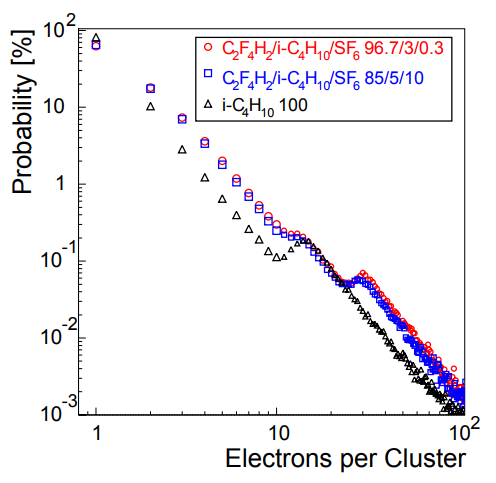
\includegraphics[width=0.65\textwidth]{RPC/cluster.png}
	\captionsetup{type=figure}\caption{Distributions du \textit{"cluster size"} pour un mélange gazeux typique utilisé pour les RPC calculées en utilisant HEED \cite{HEED}. Les particules incidentes sont des pions de \SI{7}{\giga\eV} pour le mélange avec \num{10}\% d'isobutane et \SI{120}{\giga\eV} pour le mélange avec \num{0.3}\%. La température du gaz est $T=\SI{296.15}{\kelvin}$ et la pression $p=\SI{1013}{\milli\bar}$. En coupant à \num{500} électrons et par intégration on trouve un nombre d'électrons moyen par amas de \num{1.9} pour l'isobutane, \num{2.6} pour le mélange à \num{10}\% de \chemform{SF_6} et \num{2.8} pour le mélange à \num{0.3}\% de \chemform{SF_6}.}
	\label{cluster}
\end{figure}

\subsection{Le facteur de multiplication}
Après l'ionisation, les électrons primaires vont être accélérés grâce au champ électrique entre les électrodes ce qui peut donner lieu à une avalanche. Cependant, afin d'éviter les modes \textit{streamer} et \textit{spark}, le mélange gazeux contient généralement des gaz très électronégatifs. Ceci a pour effet de capturer certains électrons primaires, les molécules très électronégatives ayant tendance à former des anions, réduisant ainsi la taille de l'avalanche. 

Tous les électrons non absorbés sont accélérés par le champ électrique et sont soumis à des chocs élastiques et inélastiques avec les autres molécules du gaz. Si l'énergie échangée lors de ces collisions est assez importante pour ioniser à son tour d'autres molécules du gaz, on assiste à une multiplication des paires électron-ion et à une réaction en cascade. Les électrons migrent vers l'anode et les cations vers la cathode mais à des vitesses beaucoup moins élevées que pour les électrons de par leur masse nettement plus importante. Ces processus ont de très grandes fluctuations stochastiques.

En définissant $\alpha$ le taux de création de paires d'ion-électron secondaires créées par unité de distance (coefficient d'ionisation de \bsc{Townsend}) et  $\beta$ le taux d'électrons capturés par unité de distance par les molécules électronégatives pour former des anions (coefficient d'attachement), il vient pour un déplacement  $\dd z$ :
\begin{equation}
	\frac{\dd \bar{n}}{\dd z}=(\alpha-\beta)\bar{n} \quad \quad \quad \frac{\dd \bar{p}}{\dd z}=\alpha\bar{n} 
\end{equation}
avec la première équation décrivant la variation du nombre moyen d'électrons et la deuxième celle du nombre moyen d'ions positifs. On peut définir également $\alpha_{eff}=\alpha-\beta$ qu'on appelle coefficient de \bsc{Townsend} effectif. En posant les conditions initiales $\bar{n}=1$ et $\bar{p}=0$, on obtient les nombres moyens d'électrons et d'ions positifs produits sur une distance $z$: 
\begin{equation}
\bar{n}=\exp(\alpha-\beta)z \quad \quad \quad \bar{p}=\frac{\alpha}{\alpha-\beta}\left(\exp^{(\alpha-\beta)z}-1\right)
\end{equation}
Le coefficient de \bsc{Townsend} dépend du champ électrique appliqué. La figure \ref{tow} montre cette dépendance pour un mélange de gaz donné.

\begin{figure}[ht!]
	\centering
	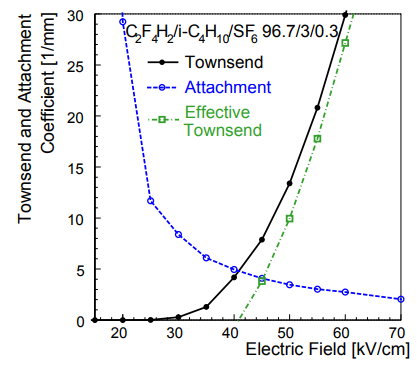
\includegraphics[width=0.62\textwidth]{RPC/tow.png}
	\captionsetup{type=figure}\caption{Coefficient de \bsc{Townsend} et coefficient d'attachement calculés grâce à Imonte \cite{imonte} pour $T=\SI{296.15}{\kelvin}$ et $p=\SI{1013}{\milli\bar}$ pour un mélange de gaz donné \cite{Riegler:570462}.}
	\label{tow}
\end{figure}

\subsection{Charges créées par l'avalanche}
La charge totale à la fin du développement du processus de multiplication peut être vue comme la somme de plusieurs avalanches qui sont indépendantes les unes des autres. Chaque amas primaire crée sa propre avalanche qui est soumise à des fluctuations statistiques.

En supposant $\alpha$ et $\beta$ constantes, la charge totale à l'emplacement $z$ peut être exprimée comme :
\begin{equation}
q(z)=\sum_{j=1}^{n_c}q_{e}M_{j}n_{j,0}\exp^{(\alpha-\beta)(z-z_0^j)}
\end{equation}
\newpage
Les fluctuations statistiques sont prises en compte par \num{4} variables aléatoires :
\begin{itemize}[label=$\bullet$]
	\item Le nombre d'amas $n_c$ qui suit une distribution poissonienne 
	\begin{equation}
	P_{clusters}(n_c=n)=\frac{(\lambda_{eff}d)^{n}}{n!}\exp^{-\lambda_{eff}d}
	\end{equation}
	avec $\lambda_{eff}=\frac{\lambda}{\phi}$ la densité linéaire moyenne d'amas, $\phi$ l'angle d'incidence de la particule incidente et $d$ l'épaisseur de la couche de gaz.
	\item La position $z_0^j$ du cluster $j$ suit la loi Gamma
	\begin{equation}
	P_{j}(z_0^j=x)=\frac{x^{j-1}\lambda_{eff}^{j}}{\Gamma(j)}\exp^{-x\lambda_{eff}} \quad 0<x<d
	\end{equation}
	\item Le nombre d'électrons $n_{0}^{j}$ dans l'amas $j$ suit la loi de distribution trouvée par le programme Heed (cf.Fig~\ref{cluster}).
	\item Le facteur $M_{j}$ qui prend en compte les fluctuations de l'avalanche et la diminution du champ électrique réduit $E/p$ ($p$ la pression du gaz) par les ions, lorsque l'avalanche devient trop importante. Ce facteur est obtenu concrètement en tirant d'une distribution de \bsc{Polya} une valeur puis en la divisant par le nombre moyen d'électrons de l'avalanche.
\end{itemize}
\vspace*{-0.2cm}
\subsection{Signal induit sur l'électronique}
\vspace*{-0.6cm}
En utilisant le théorème de \bsc{Ramo} et \bsc{Shockley} \cite{HE2001250}, il peut être montré que le courant électrique induit sur l'électronique est dû au mouvement des charges entre les électrodes qui change les lignes de champ électrique et non la quantité de charges reçue par seconde par l'électrode. C'est ce courant qui peut ensuite être traité par l'électronique de lecture.
\begin{equation}
i_{ind}(t)=-q(x/v_{d})\vec{v_{d}}\cdot \overrightarrow{E_{w}}
\end{equation}
où $\overrightarrow{E_{w}}$ est appelé champ pondéré et correspond au champ électrique du détecteur si la charge est enlevée, l'électrode mise à une tension unitaire  et toutes les autres électrodes mises à la masse. $\vec{v_{d}}$ est la vitesse de dérive des charges.

La vitesse de dérive pour les électrons dans différents mélanges de gaz est donné sur la figure \ref{drift} \cite{Riegler:570462}

\begin{figure}[ht!]
	\centering
	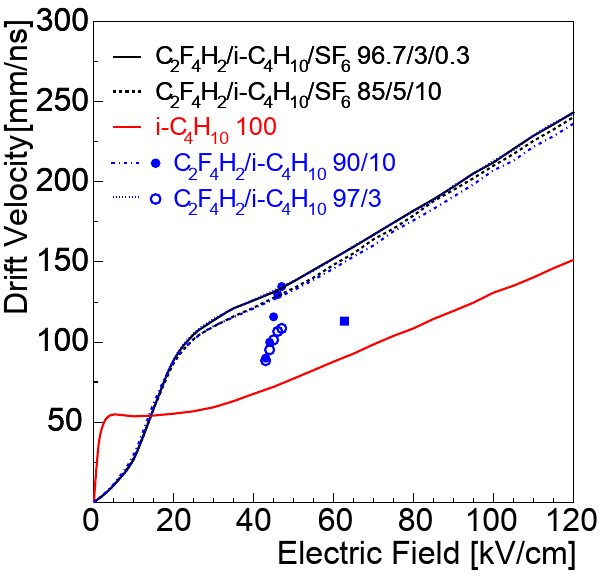
\includegraphics[width=0.60\textwidth]{RPC/drift.png}
	\captionsetup{type=figure}\caption{Vitesses de dérive calculées en utilisant le programme MAGBOLTZ \cite{MAGBOLTZ} pour différents mélanges de gaz à la température $T=\SI{296.15}{\kelvin}$ et la pression $p=\SI{1013}{\milli\bar}$.}
	\label{drift}
\end{figure}

De par leur masse beaucoup plus élevée que celles des électrons, les ions se déplacent plus lentement et participent moins au courant induit. Mettant plus de temps pour atteindre l'électrode, les ions induisent un signal plus long, ce qui accroit le temps mort du détecteur.% Ils mettent en revanche plus de temps pour atteindre l'électrode, le signal induit est donc beaucoup plus long et accroît le temps mort du détecteur.

\section{Les Resistive Plate Chambers de CMS}

Le détecteur CMS utilise des chambres double \textit{gaps} d'épaisseur \SI{2}{\milli\meter}, chacun formé par deux électrodes en Bakélite de résistivité comprise entre \SI{1e10}{\ohm\centi\meter} et \SI{6e10}{\ohm\centi\meter} (cf.Fig~\ref{cmsrpc}). 

\begin{figure}[ht!]
	\centering
	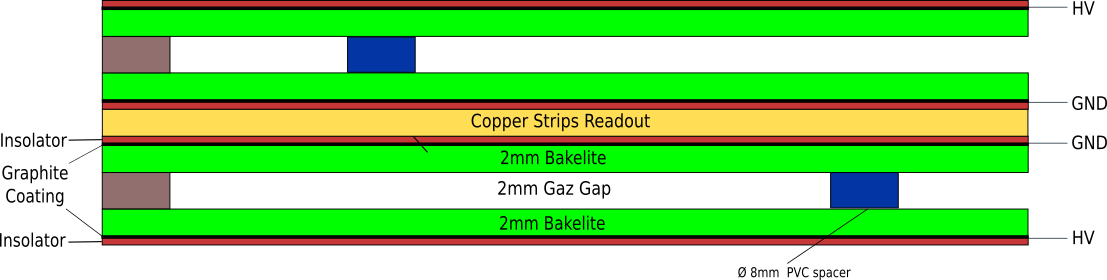
\includegraphics[width=0.90\textwidth]{RPC/CMSRPC.png}
	\captionsetup{type=figure}\caption{Schéma d'une chambre RPC dans CMS.}
	\label{cmsrpc}
\end{figure}

Afin de maintenir la distance de \SI{2}{\milli\meter} entre les électrodes, des \textit{spacers} en Polychlorure de vinyle (PVC) de \SI{8}{\milli\meter} de diamètre sont placés tous le \SI{10}{\centi\meter}. Les faces externes des électrodes sont recouvertes d'une peinture de graphite de résistance surfacique $\approx$\SI{e5}{\ohm/\sq} permettant la mise sous tension des chambres. Un film d'huile de lin de \SIrange{35}{45}{\micro\meter} d'épaisseur est appliqué sur les faces constituant les parties internes des gaps afin d'améliorer la planéité des surfaces \cite{oil} et limiter les photons ultra-violet \cite{Lu:2009zzd}. Ceci a pour effet  de réduire le bruit et le courant de fuite des RPC.
Le signal est récolté par des \textit{strips} placés entre les deux chambres et séparés de celles-ci par une couche de Mylar. Les chambres opèrent en mode avalanche pour les raisons déjà évoquées précédemment dans ce chapitre.

\subsection{Le mélange gazeux}
Le mélange gazeux utilisé par les RPC de CMS comporte :
\marginpar
{
	\centering
	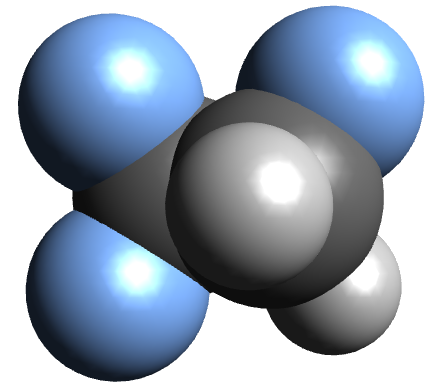
\includegraphics[width=\marginparwidth]{RPC/C2H2F4.png}
	\captionsetup{type=figure}\caption{Structure chimique du Tétrafluoroéthane.}
	\label{Tetra}
}
\marginpar
{
	\centering
	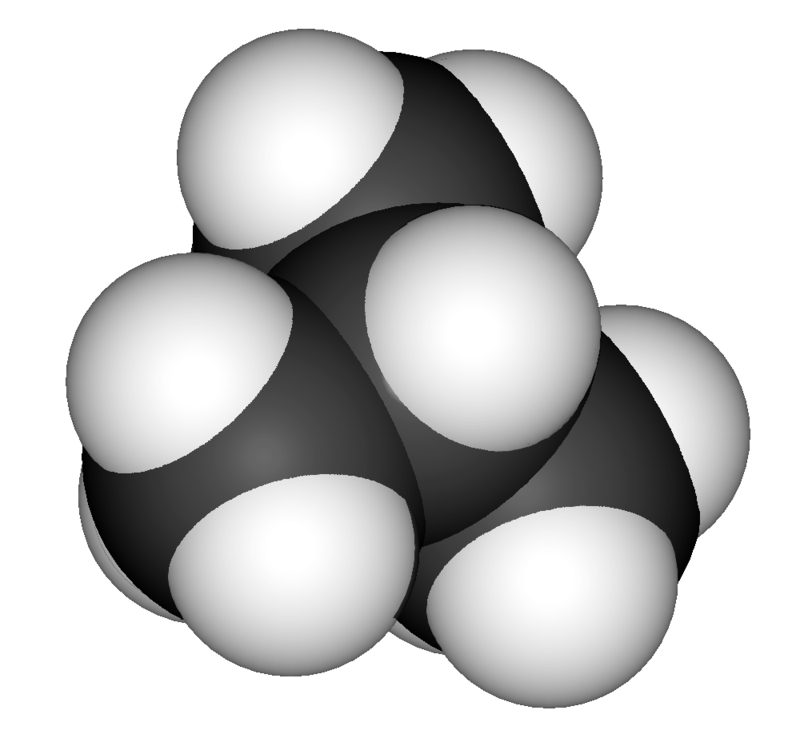
\includegraphics[width=\marginparwidth]{RPC/Isobutane.png}
	\captionsetup{type=figure}\caption{Structure chimique de l'isobutane.}
	\label{Iso}
}
\marginpar
{
	\centering
	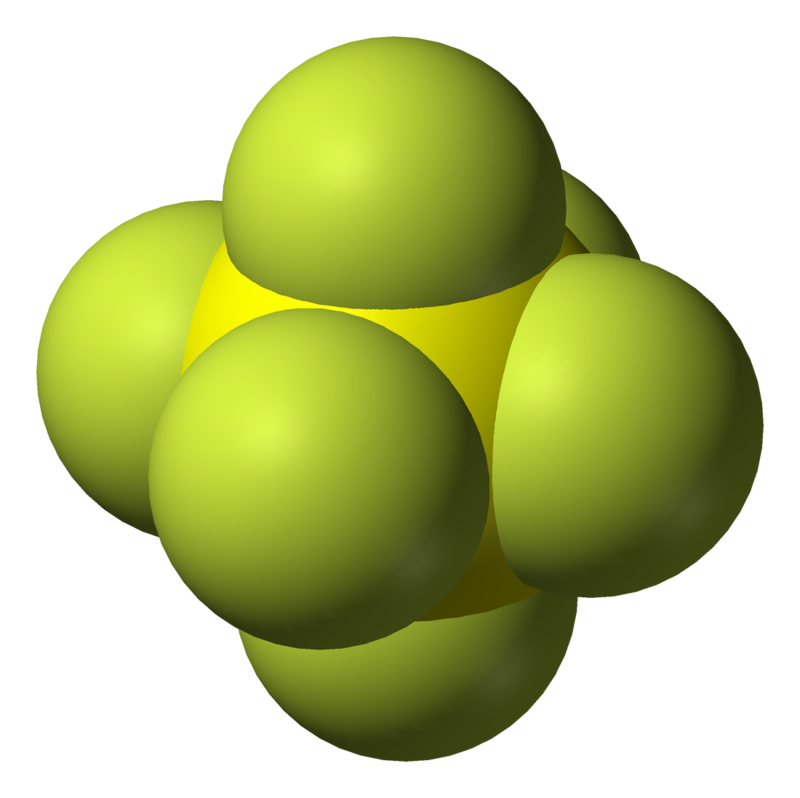
\includegraphics[width=\marginparwidth]{RPC/Sulfurhexafluoride.png}
	\captionsetup{type=figure}\caption{Structure chimique de l'hexafluorure de soufre.}
	\label{hexa}
}

\begin{itemize}[label=$\bullet$]
\item \num{95.2}\% de Tétrafluoroéthane \chemform{C_2H_2F_4} (R-134a). Composant principal du mélange, il permet une densité d'amas primaires élevée $\lambda=\SI{5.5}{\clusters\per\milli\meter}$ tout en gardant un coefficient de \bsc{Townsend} effectif élevé $\alpha_{eff}=\SI{9.15}{\per\milli\meter}$ \cite{CMS-NOTE-1997-004}.
\item \num{4.5}\% d'isobutane \chemform{iso-C_4H_{10}}, utilisé comme absorbeur de photons ultraviolets (UV) produits par la désexcitation des molécules du mélange gazeux.
\item \num{0.3}\% d'hexafluorure de soufre \chemform{SF_6}, un gaz très électronégatif, permettant de capturer l'excès d'électrons. Il participe ainsi à augmenter le coefficient d'attachement $\beta$ et permet de réduire la probabilité de \textit{streamer} \cite{Camarri:685607}.
\end{itemize}

Afin d'empêcher l'augmentation de la résistivité de la Bakélite, \num{40}\% à \num{50}\% d'humidité sont ajoutées au mélange gazeux \cite{Abbrescia:2004fv}.

Les gaz \chemform{C_2H_2F_4} et \chemform{SF_6} ont un  potentiel de réchauffement global (PRG) \footnote{Le PRG d’un gaz est le rapport entre les effets causés par la libération en début de période d’une masse donnée de ce gaz et ceux causés par la même masse de dioxyde de carbone (\chemform{CO_2}).} \textit{Global Warming Potential (GWP)} de \num{1000} et \num{23900} respectivement sur une période de \num{100} ans. Dans le but de limiter les rejets et de réduire la consommation de ces gaz, le mélange gazeux circule en circuit fermé avec une injection de gaz pur de \num{5}\% à \num{10}\% \cite{5401780}. Cependant, ces recirculations de gaz amènent à l'augmentation d'impuretés comme le \chemform{HF}, le \chemform{F^-} et d'autres types de molécules à base de Fréon \cite{1748-0221-8-08-T08003}. Une étude et un monitorage par chromatographie de la composition du gaz injecté et circulant dans les chambres sont donc nécessaires. 

\subsection{Disposition des chambres RPC dans les secteurs des bouchons de CMS}
\vspace{-0.2cm}
La disposition des chambres RPC dans CMS a été présentée dans la section \ref{RPCPRE}, page~\pageref{RPCPRE}. Celles-ci sont rectangulaires dans le tonneau et trapézoïdales dans les bouchons (cf.Fig~\ref{trap}). L'aire des strips contenus dans les chambres ainsi que leur longueur ont été optimisées afin de limiter le bruit par strip, qui pourrait augmenter la probabilité de coïncidences fortuites et être considéré comme le passage d'un muon. La longueur des strips est également limitée par le temps de propagation du signal le long de celui-ci. En effet, ce temps de propagation doit être plus court que le temps de vol entre les stations. Le changement de trajectoire du muon selon $\eta$ à cause du champ magnétique est également à prendre en compte pour la longueur des strips.

Les chambres sont donc divisées en deux (trois) $\eta-sectors$ pour les chambres du tonneau (des bouchons). Les strips ont une longueur comprise entre \num{57} et \SI{125}{\centi\meter} dans le tonneau et entre \num{39.8} et \SI{79.72}{\centi\meter} dans les bouchons. Ces trois $\eta-sectors$ sont notés $A$, $B$, $C$ selon $\eta$ décroissant et comportent \num{32} strips chacun.

Cette division le long de $\eta$ amène à la segmentation des \textit{gaps} des détecteurs afin d'extraire les signaux provenant des strips. Ainsi, les chambres des bouchons sont constituées non pas de deux mais de trois \textit{gaps} notés $i$ (\textit{Bottom gap}), $ii$ (\textit{Top Wide gap}) et $iii$ (\textit{Top Narrow gap})
 (cf.Fig~\ref{gapslayout}). 
\marginpar
{
	\centering
	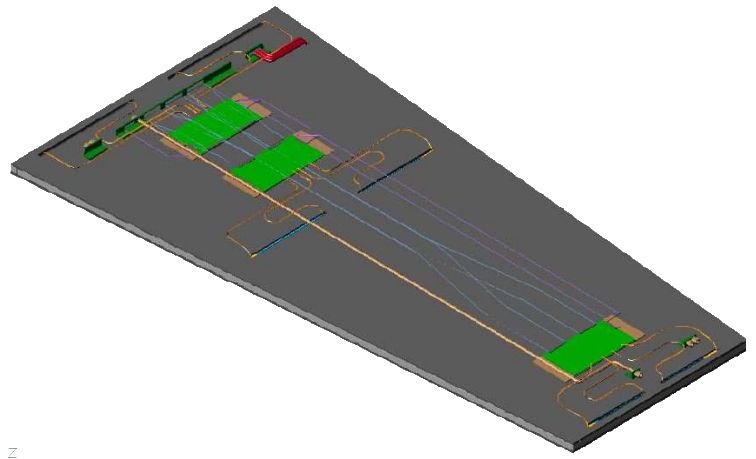
\includegraphics[width=\marginparwidth]{RPC/schemerpc.png}
	\captionsetup{type=figure}\caption{Schéma d'une chambre RPC dans les bouchons \cite{Tytgat:1477019}.}
	\label{trap}
}
\begin{figure}[ht!]
	\centering
	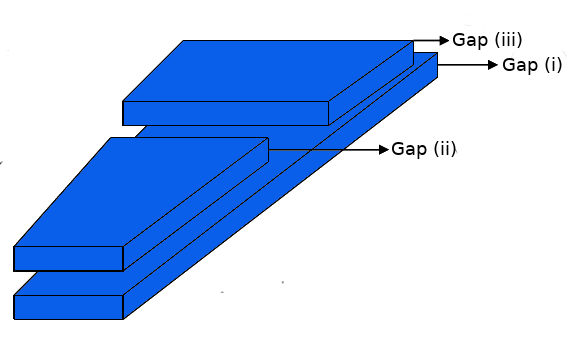
\includegraphics[width=0.50\textwidth]{RPC/gaps.png}
	\captionsetup{type=figure}\caption{Disposition des \textit{gaps} dans les chambres des bouchons \cite{gapss}.}
	\label{gapslayout}
\end{figure}

\vspace{-0.8cm}
\subsection{Électronique de lecture des chambres dans les bouchons}
\label{elecc}
\vspace{-0.2cm}
\marginpar
{
	\centering
	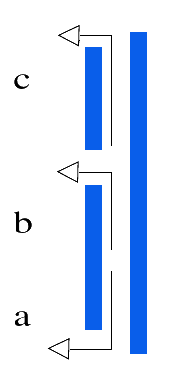
\includegraphics[width=\marginparwidth]{RPC/signalextraction.png}
	\captionsetup{type=figure}\caption{Zone d'extraction des signaux.}
	\label{extraction}
}
L'électronique de lecture des signaux provenant des strips est composée de deux types de cartes :
\begin{itemize}[label=$\bullet$]
	\item Les \textbf{Front-End Boards} (FEB) (cf.Fig~\ref{Feb}). Dans les bouchons, les FEB contiennent \num{4} ASIC appelés \textit{FEB Chips} gérant chacun les signaux de \num{8} strips qui sont connectés d'un côté grâce à des câbles coaxiaux. Le positionnement de ces FEB sur la chambre et les zones d'extraction des signaux ont été étudiés afin de limiter la gigue totale du signal (cf.Fig~\ref{extraction}). Chaque chambre comporte \num{3} FEB.
	
	\begin{figure}[ht!]
		\centering
		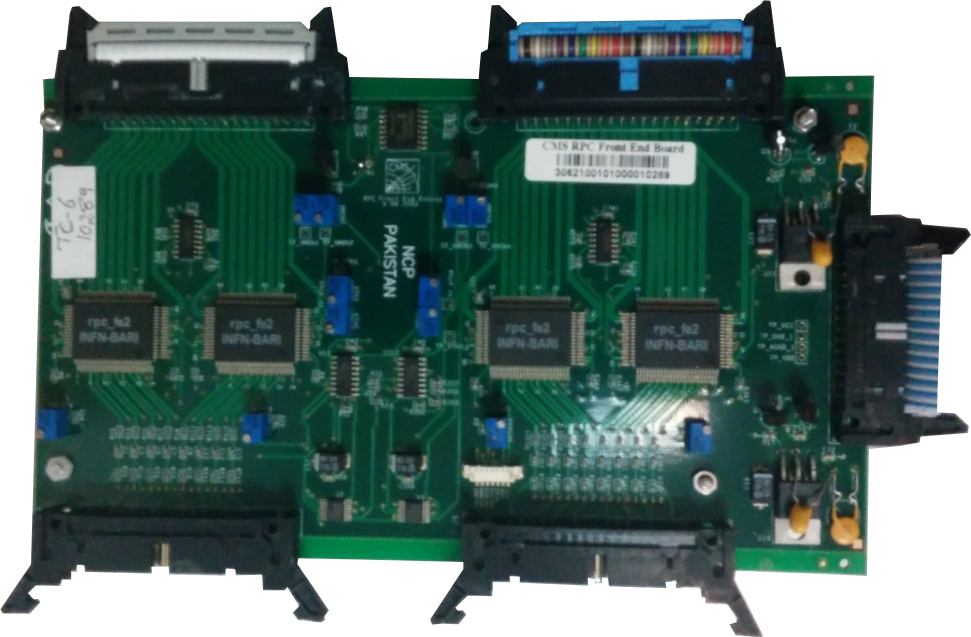
\includegraphics[width=0.35\textwidth]{RPC/Feb.png}
		\captionsetup{type=figure}\caption{Une \textit{Front-End Board }des chambres RPC dans les bouchons de CMS. Les \num{4} ASIC sont clairement visibles sur le PCB. Les strips sont reliés aux connecteurs du bas et les signaux \textit{Low-Voltage Differential Signaling} (LVDS) sont envoyés grâce aux câbles reliés aux connecteurs du haut. Le connecteur sur la droite est, quant à lui, relié au \textit{Distribution Board} (DB) et amène la basse tension et les signaux I$^2$C.}
		\label{Feb}
	\end{figure}

	Le schéma de principe de l'électronique d'une voie du FEB est donné figure \ref{schemeelec} \cite{electro}. Le signal est amplifié par un gain important variant linéairement ($\sim$\SI{2}{\milli\volt\per\femto\coulomb}) jusqu'à \SI{100}{\femto\coulomb} et un gain plus faible au delà. Un discriminateur compare ensuite le signal amplifié à une tension de seuil programmable (\SI{220}{\milli\volt} dans CMS) et permet de sélectionner la charge minimale de déclenchement. Cependant ce circuit possède un \textit{time-walk} de $\sim$\SI{10}{\nano\second} sur la gamme dynamique du signal d'entrée. Ce \textit{time-walk} est incompatible avec l'utilisation des RPC comme système de déclenchement de CMS. Afin d'obtenir une bonne résolution temporelle en limitant le \textit{time-walk}, un circuit RC différentie le signal d'entrée et l'envoie dans un \textit{zero-crossing discriminator}. Ces deux signaux sont ensuite envoyés dans un circuit de coïncidence. Cette méthode permet de réduire le \textit{time-walk} à $\sim$\SI{1}{\nano\second}. Le signal en sortie déclenche ensuite un circuit monostable qui définit la largeur réglable du signal de sortie. La largeur de ce signal a été réglée à $\sim$\SI{100}{\nano\second} afin de ne pas déclencher sur les rebonds du signal d'entrée qui pourraient survenir étant donné qu'il n'y a pas d'adaptation d'impédance au bout des strips. Finalement, le signal sort par transmission différentielle basse-tension \textit{Low-Voltage Differencial Signaling} (LVDS) grâce à des paires de câbles torsadés. Chaque FEB possède au moins un capteur de température afin de vérifier le bon fonctionnement de la carte.
	
	\begin{figure}[ht!]
		\centering
		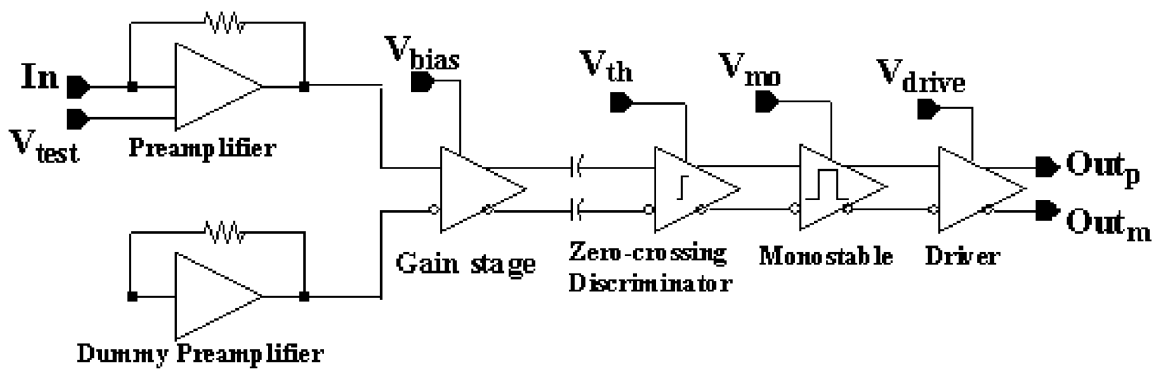
\includegraphics[width=0.90\textwidth]{RPC/schemeelec.png}
		\captionsetup{type=figure}\caption{Schéma de principe de l'électronique d'une voie du FEB.}
		\label{schemeelec}
	\end{figure}
	
	\item Les \textbf{Distribution Board} (DB) (cf.Fig~\ref{DB}) permettent de configurer et de monitorer grâce à une interface \textit{Inter-Integrated Circuit} (I$^2$C) les paramètres des FEB. Ces paramètres sont la tension de seuil du discriminateur (\textit{Threshold Voltage} $V_{Th}$) et la largeur du signal de sortie (\textit{Monostable Voltage} $V_{Mon}$). Ces paramètres sont communs aux \num{8} voies d'un même ASIC d'un FEB. Les valeurs par défaut de ces paramètres\footnote{En cas de perte de connexion.} sont réglables par des potentiomètres placés sur le PCB des FEB, pour les FEB servant de test. Pour les FEB présents dans les chambres de CMS, ces potentiomètres ont été remplacés par des convertisseur digital analogique (DAC). Chaque chambre des bouchons possède un DB. Les DB fournissent aussi la basse tension aux FEB.
	
		\begin{figure}[ht!]
		\centering
		\includegraphics[width=0.35\textwidth]{RPC/DB.png}
		\captionsetup{type=figure}\caption{Un DB permettant les configurations des paramètres des FEB par I$^2$C ainsi que leur alimentation.}
		\label{DB}
	\end{figure}

\end{itemize}

\subsection{Point de fonctionnement des RPC}
\vspace{0.3cm}
Afin d'obtenir le meilleur point de fonctionnement pour chaque chambre RPC de CMS, des scans en tension sont effectués à chaque début du redémarrage annuel.

Les hautes tensions $H_{eff}$ sont choisies de manière équidistante dans la gamme \\ $[\SI{8600}{\volt}, \SI{9800}{\volt}]$ avec :
\begin{equation}
HV_{eff}(P,T)=HV\frac{P_0}{P}\frac{T}{T_0}
\end{equation}
Cette tension effective tient compte de la variation de température et de pression dans la caverne.

Ces scans sont ensuite analysés. Les courbes d'efficacité obtenues sont ajustées par une sigmoïde.

\begin{equation}
\epsilon=\frac{\epsilon_{max}}{1+e^{-\lambda\left(HV_{eff}-HV_{50\%}\right)}}
\end{equation}

Les trois paramètres de l'ajustement sont l'efficacité maximale $\epsilon_{max}$, la tension $HV_{50\%}$ pour laquelle l'efficacité d'ajustement est égale à \num{50}\%, et la pente $\lambda$ de la sigmoïde au point $HV_{50\%}$, définie par :

\begin{equation}
\lambda=\frac{4}{\epsilon_{max}}\frac{\dd \epsilon}{\dd \left(HV_{eff}\right)}
\end{equation}

Le point de fonctionnement $H_{work}$ est ensuite défini par $HV_{knee}+\SI{120}{\volt}$ ($HV_{knee}+\SI{100}{\volt}$) dans les bouchons (le tonneau), où $HV_{knee}$ est la tension pour laquelle l'ajustement donne une efficacité de \num{95}\%.

La figure \ref{working} montre le point de fonctionnement moyen, l'efficacité moyenne au point de fonctionnement et la tension moyenne pour laquelle l'efficacité est de \num{50}\% pour les différents scans en tension effectués depuis \num{2011}.
\vspace{0.5cm}
\begin{figure}[ht!]
	\centering
	\subfloat[Pour le tonneau.]{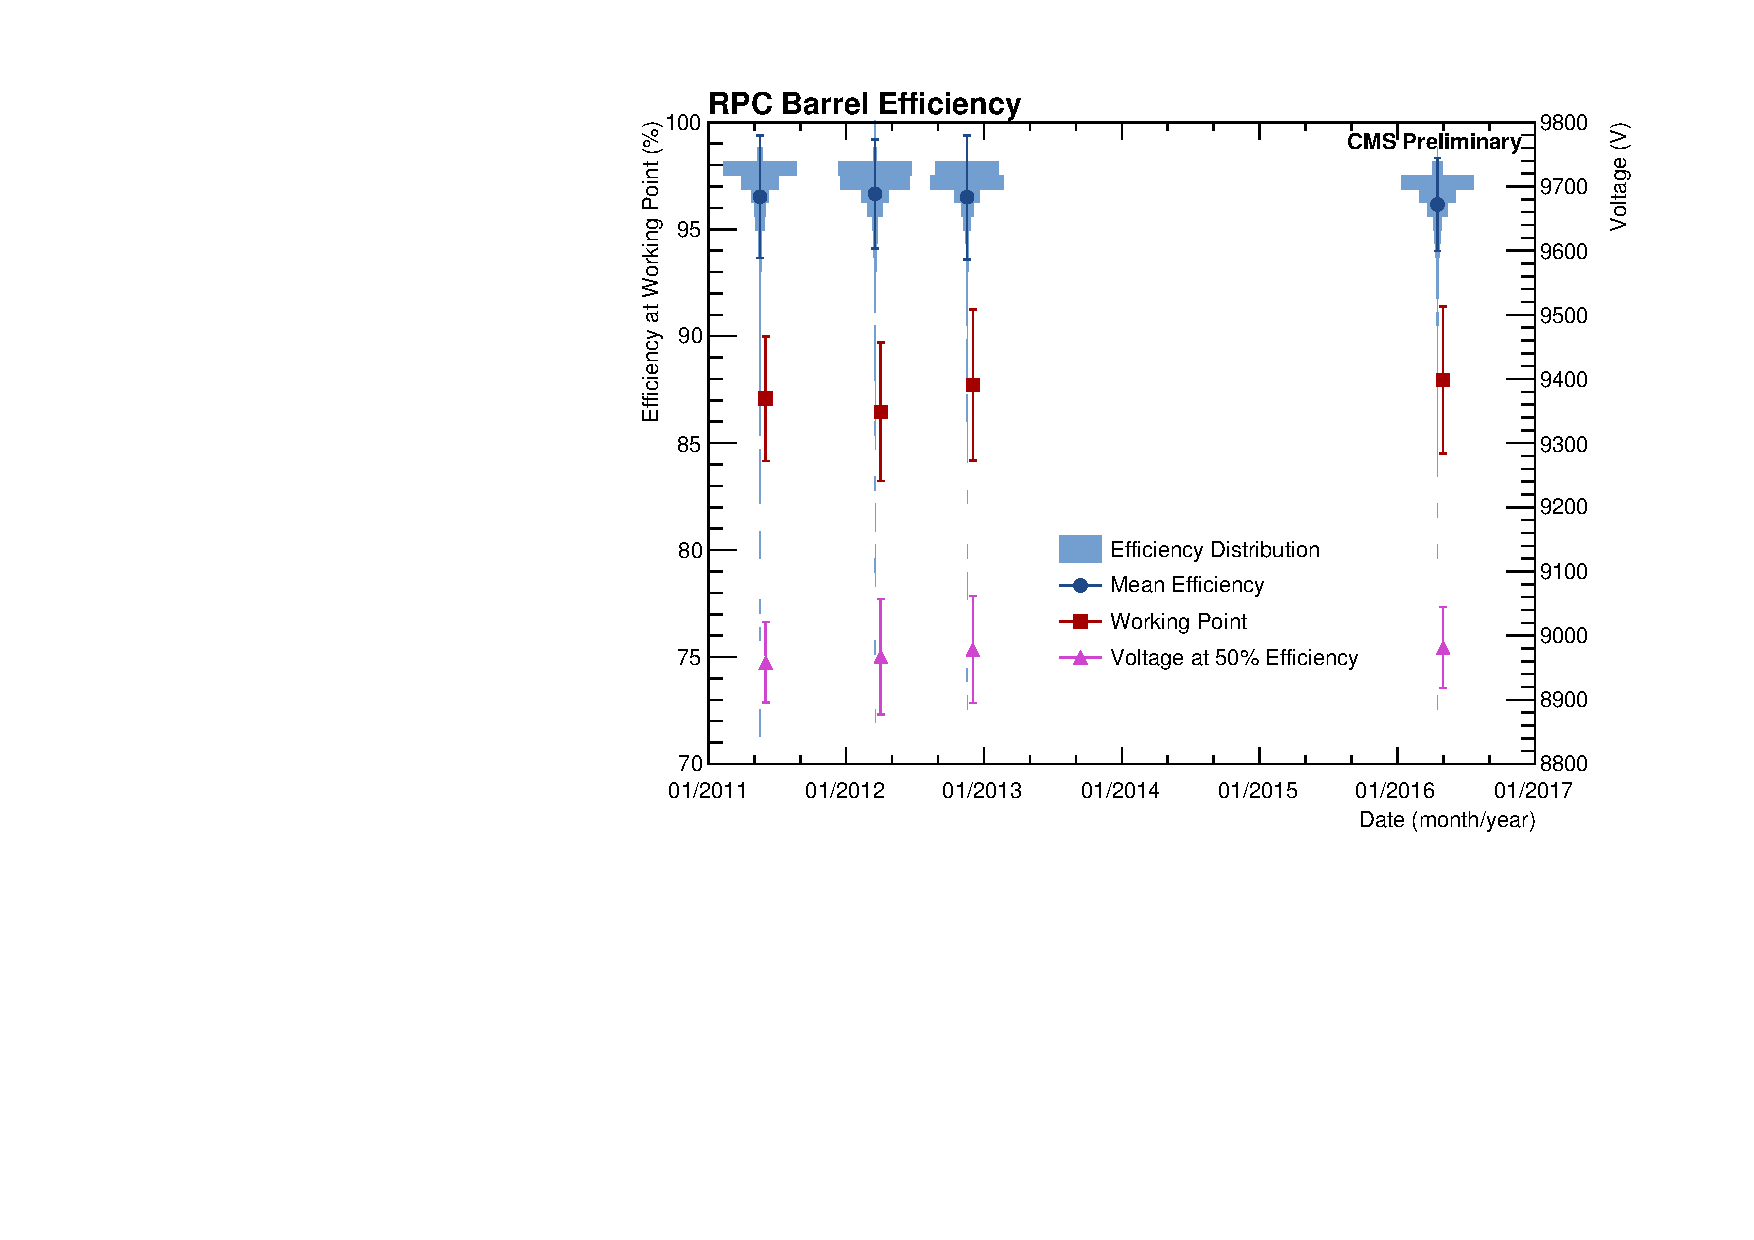
\includegraphics[width=.50\linewidth]{RPC/barrel.pdf}}
	\hfill
	\subfloat[Pour les bouchons.]{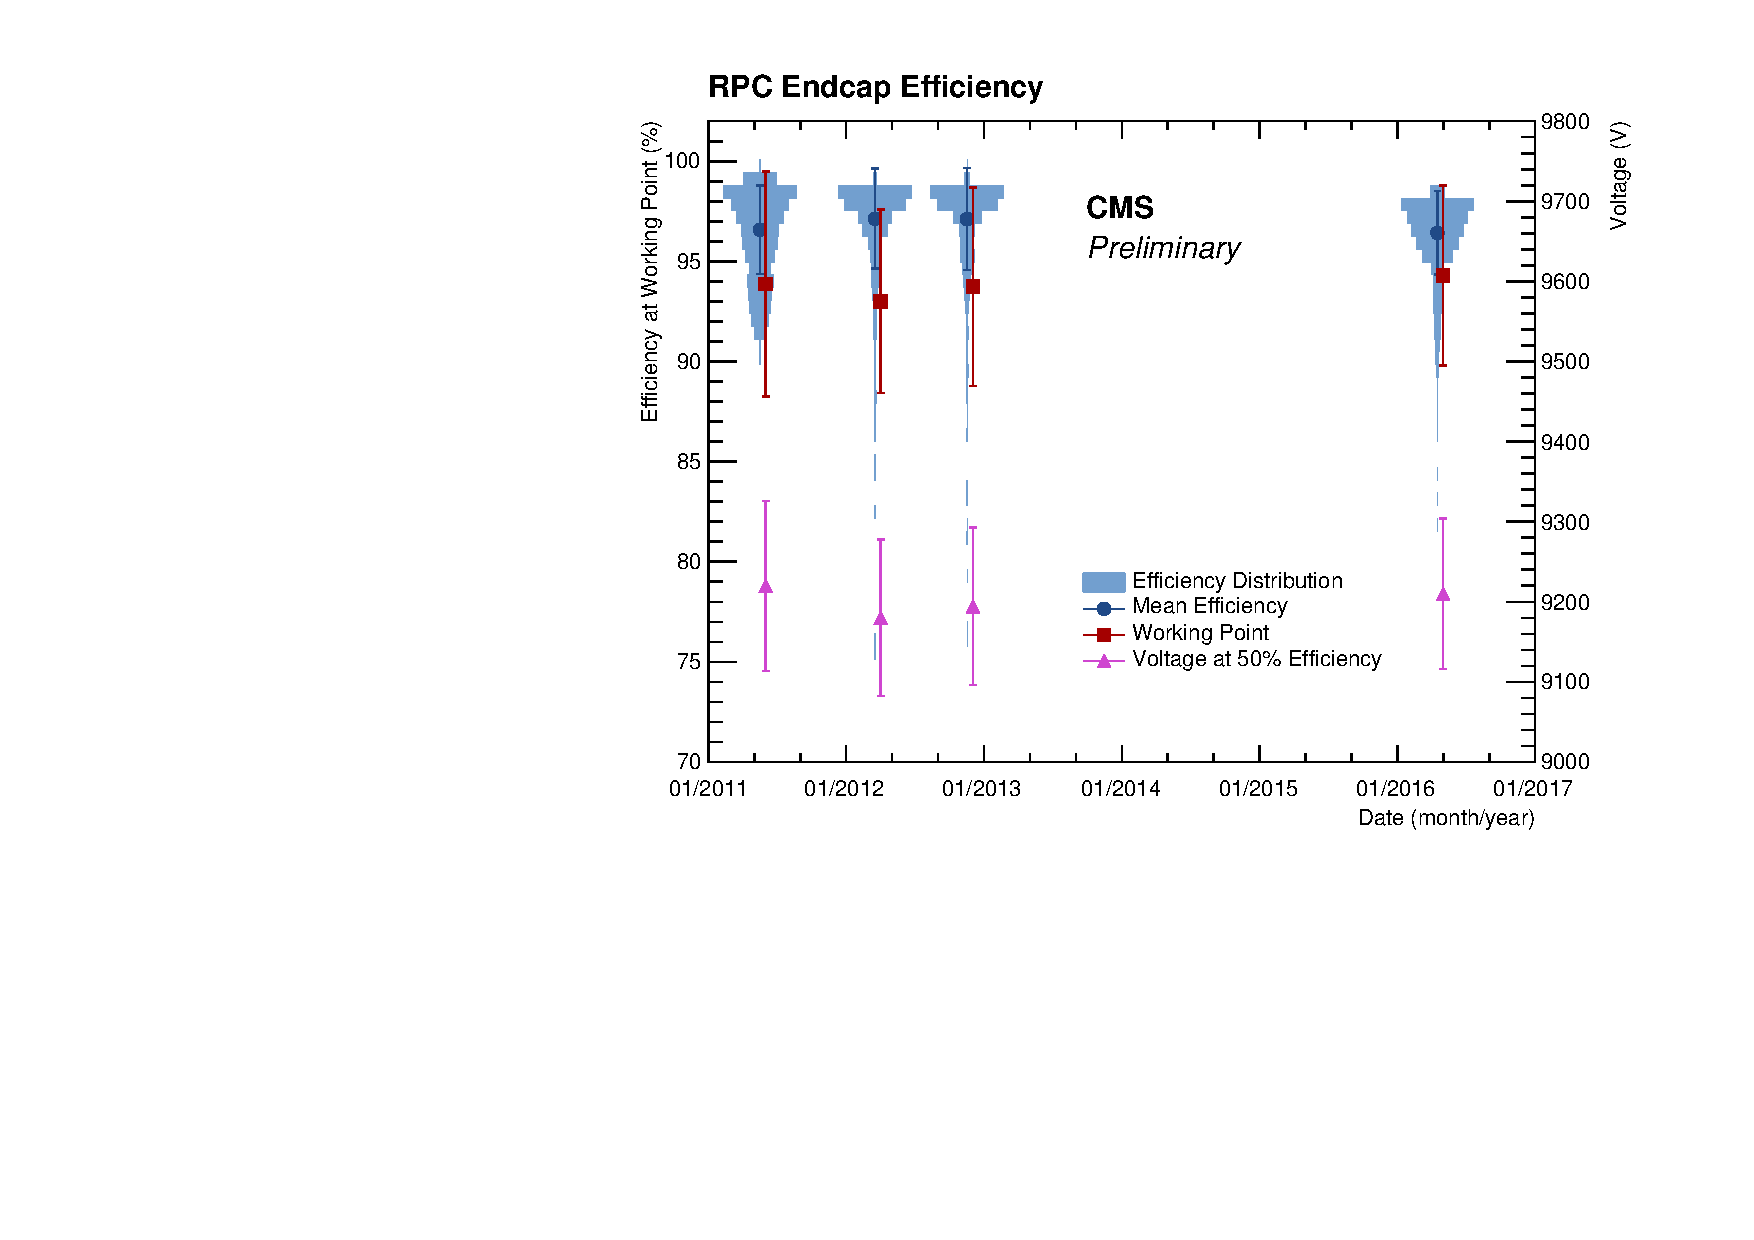
\includegraphics[width=.50\linewidth]{RPC/endcap.pdf}}
	\caption{Point de fonctionnement moyen, efficacité moyenne au point de fonctionnement et tension moyenne pour laquelle l'efficacité est de \num{50}\% pour les différents scans en tension effectués depuis \num{2011} \cite{working2}.}
	\label{working}
\end{figure}
\newpage
\section{Mise à niveau des RPC pour la Phase-2 de CMS}
Avec le passage du LHC au HL-LHC vers 2026, la luminosité est prévue pour être multipliée par un facteur \num{5} à \num{7.5} et le nombre d'événements \textit{pile-up} devrait passer de $\sim 40$ à $\sim 140$ voire $\sim 200$. Afin de maintenir les performances de CMS, celui-ci doit également être mis à niveau. Certaines de ces améliorations ont été détaillées dans le chapitre précédent. La mise à niveau du trajectographe à muons a fait l'objet de nombreuses études compilées dans le TDR \textit{The \textbf{Phase II} Upgrade of the CMS Muon Detectors} \cite{Lourenco:2283189}. Les tests de vieillissement effectués montrent que la plupart des chambres du trajectographe à muons seront capables de résister à l'environnement du HL-LHC jusqu'à la fin de la Phase-2 prévue en \num{2038} sans une perte significative de l'efficacité. Pour ce qui concerne les chambres RPC des bouchons, les mises à niveaux notables sont :

\begin{itemize}[label=$\bullet$]
	\item Le changement du \textit{Link System} des RPC responsable de l'envoi des données des chambres RPC au système de déclenchement et au système de lecture des données. Le \textit{Link System} actuel possède des éléments qui peuvent être perturbés par des bruits électromagnétiques et ne sont pas certifiés pour toute la durée de vie du HL-LHC. De plus le système actuel enregistre les temps des \textit{hits} avec une résolution temporelle de \SI{25}{\nano\second}, synchronisée avec les croisements de faisceaux de CMS, ce qui est un ordre de grandeur au dessus de la résolution des chambres RPC $\sim\SI{1.5}{\nano\second}$. Le nouveau système enregistrera les \textit{hits} avec une résolution de \SI{1}{\nano\second}. Cette amélioration permettra notamment de supprimer les \textit{hits} de bruit arrivant hors temps et de faciliter la synchronisation du système des RPC. Un déclenchement pour la détection d'hypothétiques particules chargées lourdes et stables, \textit{Heavy Stable Charged Particles} (HSCP) est également en cours d'étude \cite{Lourenco:2283189}.
	
	\item L'instrumentation des régions RE3/1 et RE4/1 (cf.Fig~\ref{end}) par des RPC de nouvelle génération. Ces chambres permettront d'étendre l'acceptance géométrique de $|\eta|=\num{1.9}$ à  $|\eta|=\num{2.4}$. L'instrumentation de ces zones a été prévue dès le début de CMS, mais n'avait pas été réalisée à cause des flux de particules importants présents dans ces zones. 
	
	En ajoutant les chambres RPC dans les zones RE3/1 et RE4/1 aux CSC déjà présents, la résolution temporelle sera améliorée d'un facteur deux (cf.Fig~\ref{intrasec}) \cite{Lourenco:2283189}.
	
	\begin{figure}[ht!]
		\centering
		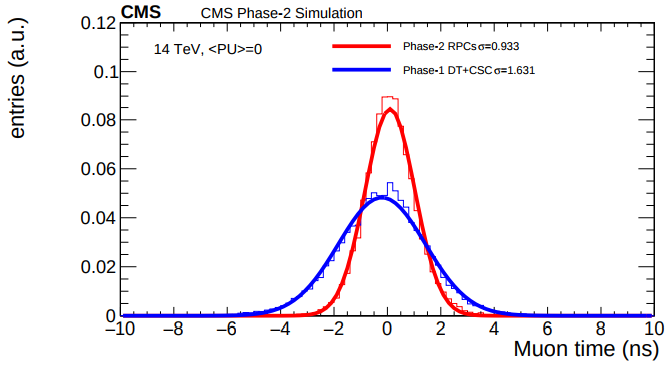
\includegraphics[width=0.90\textwidth]{RPC/intrasec.png}
		\captionsetup{type=figure}\caption{Résolution temporelle simulée pour des traces de muons dans la région vers l'avant, dans le cas où seules sont présentes les chambres CSC et DT (bleu), et dans le cas ou les chambres RPC des zones RE3/1 et RE4/1 sont incluses (rouge) \cite{Lourenco:2283189}.}
		\label{intrasec}
	\end{figure}
	Les nouvelles chambres RPC, \textit{improved RPC} (iRPC) auront une meilleure résolution spatiale (de l'ordre de quelques centimètres) le long des \textit{strips} \footnote{La courbure de la trajectoire causée par le champ magnétique n'est pas prise en compte.} en utilisant un PCB permettant une lecture des \textit{strips} des deux côtés. Ce type de lecture et de PCB est l'object du chapitre \ref{time} de cette thèse.
	\newpage
	Bien que les CSC puissent identifier et déclencher sur des muons dans la région des bouchons avec une efficacité élevée, ces chambres sont moins efficaces dans certaines zone en $|\eta|$ à cause des \textit{spacers} dans les chambres. En incluant les hits des RPC dans l'algorithme de recherche de segment élémentaire pour le \textit{trigger}, il est possible de récupérer une bonne efficacité dans ces zones (cf.Fig~\ref{effii}). Il est également possible de lever les ambiguïtés des hits CSC (\textit{ghosts})  au niveau du \textit{trigger} L1.
	
	\begin{figure}[ht!]
	 	\centering
	 	\subfloat[Pour la station \num{3}.]{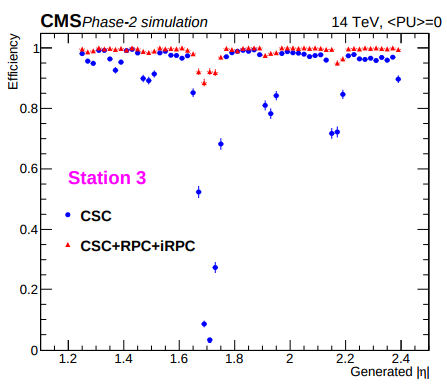
\includegraphics[width=.70\linewidth]{RPC/effstation3.png}}
	 	\\
	 	\subfloat[Pour la station \num{4}]{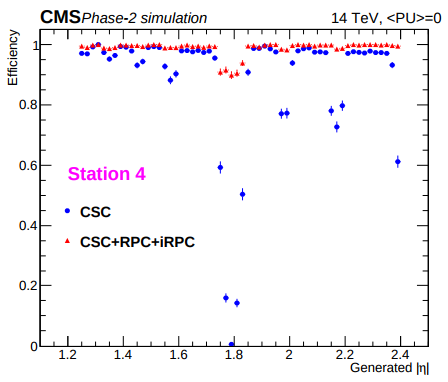
\includegraphics[width=.70\linewidth]{RPC/effstation4.png}}
	 	\caption{Impact de l'inclusion des \textit{hits} provenant des chambres RPC sur l'efficacité du déclenchement local dans les stations \num{3} (haut) et \num{4} (bas). La contribution des iRPC débute à partir de $|\eta|=\num{1.8}$ \cite{Lourenco:2283189}.}
	 	\label{effii}
	 \end{figure}
	
	Les chambres RPC, dans les zones RE3/1 et RE4/1, augmentent également la redondance dans la zone des bouchons. Ceci permet d'assurer une détection des muons même en cas de défaillance d'une ou plusieurs chambres CSC.
\end{itemize}

\subsection{Les iRPC retenues par le TDR}
De nombreux types de chambres différents ont été testés afin de vérifier leurs caractéristiques et de déterminer s'ils étaient de bons candidats en vue de l'instrumentation des zones RE3/1 et RE4/1 \cite{Lourenco:2283189}.

Dans ce but, durant cette thèse, des chambres construites à partir de verres de basse résistivité (\SI{1e11}{\ohm\centi\meter}), de taille $\num{32}\times\SI{30}{\square\centi\meter}$ ont été testées. La caractérisation de ces chambres est l'objet du chapitre \ref{glagla}.


Le type de chambre retenu par le TDR comme solution privilégiée est la chambre double \textit{gaps} d'épaisseur \SI{1.4}{\milli\meter} construite avec des électrodes en Bakélite de résistivité comprise entre \SI{0.9e10}{\ohm\centi\meter} et \SI{3.0e10}{\ohm\centi\meter} et d'épaisseur \SI{1.4}{\milli\meter} développées par nos collègues de Kodel. Un PCB, développé par l'IPNL et qui sera décrit au chapitre \ref{time}, permet la lecture des \textit{strips} des deux côtés. Il est placé entre ces électrodes. 

La figure \ref{datairpc} donne l'efficacité et la taille moyenne d'un amas on fonction de la tension effective appliquée, en l'absence et en présence d'un flux de gammas de \SI{1.91}{\kilo\hertz\per\square\centi\meter}. Le déplacement du point de fonctionnement est inférieur à \SI{300}{\volt} et l'efficacité reste autour des \num{95}\% même en présence du flux de gammas. La chambre utilisée pour ces résultats est de forme trapézoïdale (grande base : \SI{92}{\centi\meter}, petite base : \SI{63}{\centi\meter}, longueur : \SI{166.3}{\centi\meter}) avec une électronique à \textit{strips} de \SI{2}{\centi\meter} de largeur\footnote{Cette électronique n'est pas la solution privilégiée par le TDR.}\cite{Lourenco:2283189}.

\begin{figure}[ht!]
	\centering
	\subfloat[En l'abscence de flux de gammas.]{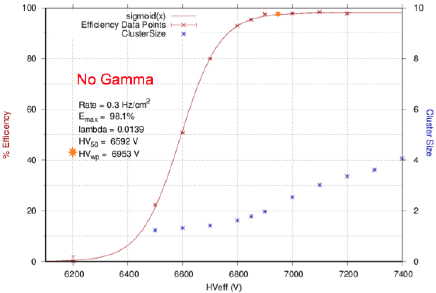
\includegraphics[width=.65\linewidth]{RPC/nogamma.png}}
	\\
	\subfloat[En présence d'un flux de gammas de \SI{1.91}{\kilo\hertz\per\square\centi\meter}.]{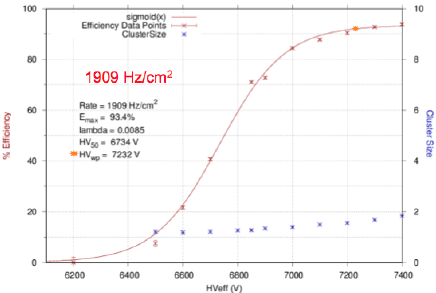
\includegraphics[width=.65\linewidth]{RPC/gamma.png}}
	\\
	\caption{Efficacité et taille moyenne d'un amas en fonction de la tension appliquée \cite{Lourenco:2283189}.}
	\label{datairpc}
\end{figure}

